\documentclass[12pt,a4paper]{article}
\usepackage{graphicx}
\usepackage{gensymb}
\usepackage{amsmath}
\usepackage{amssymb}
\usepackage{bm}
\usepackage{tikz}
\usepackage{titlesec}
\usepackage{float}
\usepackage{mathtools}
\usepackage{caption}
\usepackage{subcaption}
\usepackage{minted}
\setminted{frame=single,framesep=10pt,breaklines,linenos}
\setcounter{secnumdepth}{4}
\allowdisplaybreaks
\tikzset{
    node distance=2cm, % specifies the minimum distance between two nodes. Change if necessary.
    }
\title{Case Study Modelling an Electronic Component}
\author{
  Azure Hutchings
  \and
  Jean-Luc Danoy
  \and
  Faris Saad S Alsubaie
}
\date{28 October 2019}
 
\begin{document}
 
\begin{titlepage}
\maketitle
\end{titlepage}

\pagebreak

\tableofcontents

\pagebreak

\section{Introduction}

\subsection{Purpose of the Report}
The following report investigates the steady-state heat distribution in a newly designed component. 
\\\\
The report will discuss how to numerically solve for the steady-state heat distribution in the newly designed component, to ensure it will perform to all the specifications. The report will also discuss the development of the mathematical model of the heat distribution in the component and discuss the efficiency of different methods and the effect of different ambient temperatures.

\subsection{Mathematical Model}
\begin{figure}[H]
	\center
	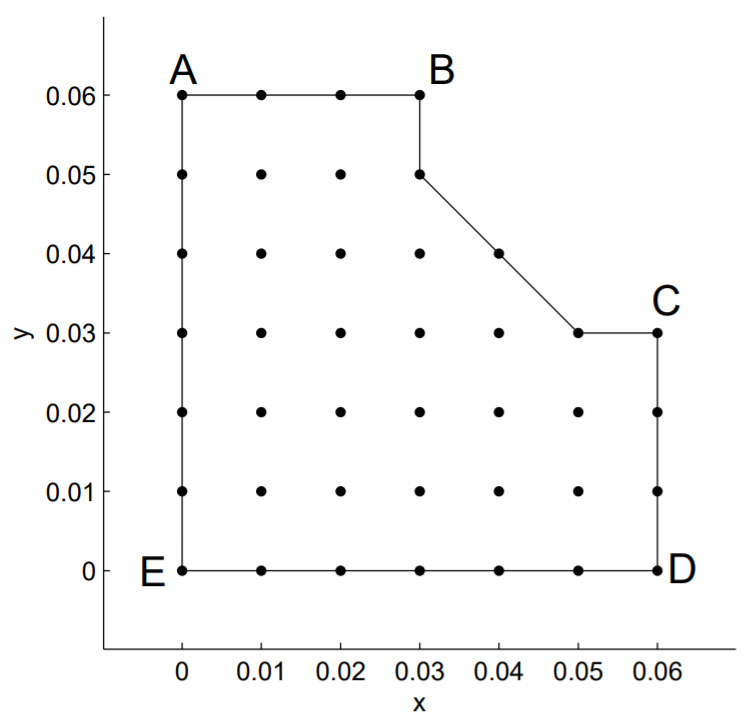
\includegraphics[width=0.9\linewidth]{images/Component.png}
	\caption{Schematic of electronic component.}
	\label{fig:componentSchematic}
\end{figure}
The component schematic is shown in Figure \ref{fig:componentSchematic}. The location of the component within the device means it's subject to different temperature condition along it's boundaries. The boundary A-B is in perfect thermal contact with another component which the temperature is known to $70\degree$C. The boundary C-D is also in perfect thermal contact with another component which the temperature is known to be $40\degree$C. The boundary A-E-D is thermally insulated and the boundary B-C is exposed to the air at ambient temperature.
\\\\
This type of model can be described with Laplace's equation. Letting $T(x,y)$ represent the temperature of the component at point $(x, y)$, the model is as follows	

\begin{center}
\begin{tabular}{c c}
$\frac{\partial^2 T}{\partial x^2}+\frac{\partial^2 T}{\partial y^2}=0$ & in the interior\\
$T = 70$ & on boundary A-B \\
$T = 40$ & on boundary C-D \\
$\boldsymbol{\nabla} T \cdot {\hat{\textbf{n}}} = 0$ & on boundary A-E-D\\
$k\boldsymbol{\nabla}T\cdot\hat{\textbf{n}} = h(T_{\infty} - T)$ & on boundary B-C
\end{tabular}
\end{center}
Where the thermal conductivity is $k=3Wm^{-1}C^{-1}$, and the heat transfer coefficient is $h=20 Wm^{-2}C^{-1}$. To begin with, we will assume the ambient temperature is $T_\infty = 20$.
\clearpage
\section{Method for Discretising the Problem}
If this was left as a continuous partial differential equation, we would need to analytically solve it. However, it can be much quicker to numerically solve this problem and still retain a high degree of accuracy with the final answers. In this section we will show how we converted the analytical problem to a numerical problem, how the mesh was constructed, the node ordering used, the linear system we derived from the mesh and discuss the matrix that was created from it.


\subsection{Constructing the Finite Difference Mesh}
Suppose we had a function $\phi(x,y,t)$ which gives the temperature at the point (x,y) on a 2-dimensional plane where t is the time since the start of the initial conditions. If the function has a steady-state solution, then it means at some point in time, any increase in time will not result in a change of temperature. This means that 
\begin{center}
$\frac{d\phi}{dx}|_{x_i}\approx\frac{\phi(x_i+\Delta x)-\phi(x_i)}{\Delta x}$,
\end{center}
where the change in $x$ along $\phi$ at the point $x_i$ is approximately the functions forward difference over the distance between nodes. We can then take the derivative of this again using backwards difference to get the second derivative centred around $x_i$.
\begin{center}
$\frac{d^2\phi}{dx^2}|_{x_i}\approx\frac{\phi(x_i+\Delta x)-2\phi(x_i)+\phi(x_i-\Delta x)}{(\Delta x)^2}$,
\end{center}
If we do the same for the change in $y$, we arrive at an analogous equation
\begin{center}
$\frac{d^2\phi}{dy^2}|_{y_i}\approx\frac{\phi(y_i+\Delta y)-2\phi(y_i)+\phi(y_i-\Delta y)}{(\Delta y)^2}$,
\end{center}
To numerically solve this problem, a finite difference mesh must be constructed and a matrix must be created to represent this information.
\\\\
By splitting the component up into intervals of 0.01 in both the $x$ and $y$ direction, the component can be split into a $7 \times 7$ grid. Because we know that the temperature on the upper and right hand boundaries are fixed temperatures, we can ignore them in our discretisation as nodes. They will come into effect later as the right hand side matrix. Given the previous mesh from the introduction, we can label each node u$_{i,j}$ for $i,j = 0$ to 6 where $i, j$ are given by the row and column of the node starting from the bottom left hand corner. Replacing $\phi(x,y,t)$ with $u_{i,j}(t)$ and noting that $\Delta x = \Delta y$, we arrive at the set of equations for the change in $u_{i,j}(t)$.
\begin{center}
$u'_{i,j}(t)\approx\frac{D}{\Delta x^2}\big{(}-u_{i+1,j}(t)-u_{i,j+1}(t)+4u_{i,j}(t)-u_{i-1,j}(t)-u_{i,j-1}(t)\big{)}.$
\end{center}
Note that since we are finding a state where the temperature does not change in time $(u'_{i,j}(t)=0)$, and assuming that $D\neq0$, we can rewrite this to be
\begin{center}
  $0=\big{(}-u_{i+1,j}-u_{i,j+1}+4u_{i,j}-u_{i-1,j}-u_{i,j-1}\big{)}.$
\end{center}
There are 3 different types of mesh that need to be created. These are for the A-E-D boundary, the interior of the mesh, and on the B-C boundary.
\subsubsection{Interior Nodes}
On the interior of the mesh, each node contains 4 other nodes adjacent to it, and the change in temperature at that node is given by the equation
\begin{center}
\[\frac{\partial^2 T}{\partial x^2}+\frac{\partial^2 T}{\partial y^2}=0\]
\[\frac{2T-T_W-T_E}{(0.01)^2}+\frac{2T-T_N-T_S}{(0.01)^2}=0\]
\[4T-T_W-T_E-T_N-T_S=0\]
\end{center}
\begin{center}
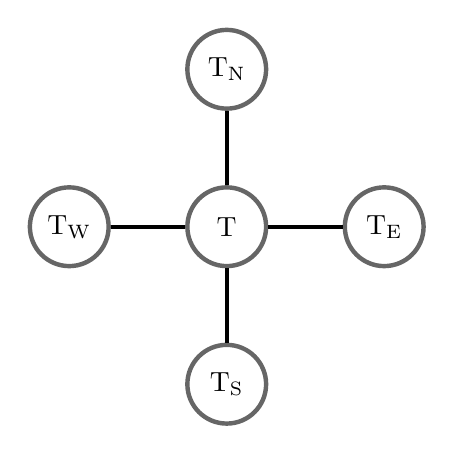
\begin{tikzpicture}[
roundnode/.style={circle, draw=black!60, ultra thick,  minimum size=10mm},
]
\node[roundnode] (center) {T};
\node[roundnode] (left) [left of=center] {T$_\text{W}$};
\node[roundnode] (right) [right of=center] {T$_\text{E}$};
\node[roundnode] (above) [above of=center] {T$_\text{N}$};
\node[roundnode] (below) [below of=center] {T$_\text{S}$};

\draw[ultra thick,-] (left.east) -- (center.west);
\draw[ultra thick,-] (above.south) -- (center.north);
\draw[ultra thick,-] (right.west) -- (center.east);
\draw[ultra thick,-] (below.north) -- (center.south);
\end{tikzpicture}
\end{center}
As an example, the node $T_{(1,1)}$ can be examined.
\begin{center}
  $4T_{(1,1)}-T_{(0,1)}-T_{(2,1)}-T_{(1,2)}-T_{(1,0)}=0$
\end{center}
\subsubsection{Boundary A-E-D Nodes}
On the boundary A-E-D, there are no nodes outside of the matrix. We can approximate them using first order forward differences (to keep the $A$ matrix SPD). This approximation can be done using the rule $\boldsymbol{\nabla} T \cdot {\hat{\textbf{n}}} = 0$, where ${\hat{\textbf{n}}}$ is the normal unit vector at the node $T$ and $\boldsymbol{\nabla} T$ is the directional gradient at $T$. The first order differences are then used to construct a finite difference equations for each node on the boundary.\\We will provide 3 examples that show all the unique cases along the boundary A-E-D, namely on the border A-E (not including A or E), the border E-D (not including E or D) and the node E.
\paragraph*{Nodes A-E}
On the A-E nodes, the normal unit vector will face directly west.
\begin{center}
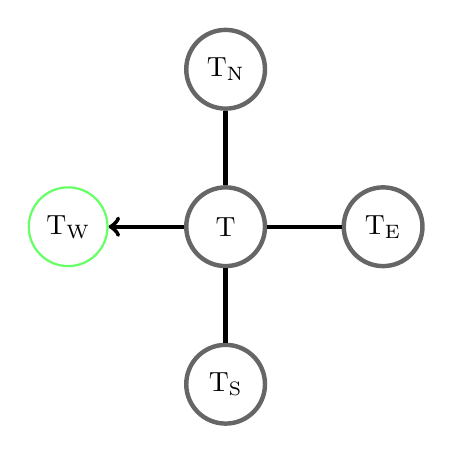
\begin{tikzpicture}[
roundnode/.style={circle, draw=black!60, ultra thick,  minimum size=10mm},
ghostnode/.style={circle, draw=green!60, thick, minimum size = 10mm},
]
\node[roundnode] (center) {T};
\node[ghostnode] (left) [left of=center] {T$_\text{W}$};
\node[roundnode] (right) [right of=center] {T$_\text{E}$};
\node[roundnode] (above) [above of=center] {T$_\text{N}$};
\node[roundnode] (below) [below of=center] {T$_\text{S}$};

\draw[ultra thick,<-] (left.east) -- (center.west);
\draw[ultra thick,-] (above.south) -- (center.north);
\draw[ultra thick,-] (right.west) -- (center.east);
\draw[ultra thick,-] (below.north) -- (center.south);
\end{tikzpicture}
\end{center}
Therefore $\hat{\textbf{n}} = (-1,0)^T$. We can construct a first order forward difference approximation for $T_W$.
\begin{center}
\[\bigg{(}\frac{\partial T}{\partial x},\frac{\partial T}{\partial y}\bigg{)}\cdot (-1,0)^T = 0\]
\[-\frac{\partial T}{\partial x} = 0\]
\[\frac{T-T_W}{0.01} = 0\]
\[T_W = T.\]
\end{center}
This value of $T_W$ can be used in the stencil around the point T.
\begin{center}
\[\frac{\partial^2 T}{\partial x^2}+\frac{\partial^2 T}{\partial y^2}=0\]
\[\frac{2T-T_W-T_E}{(0.01)^2}+\frac{2T-T_N-T_S}{(0.01)^2}=0\]
\[2T-T_W-T_E+2T-T_N-T_S=0\]
\[4T-T-T_E-T_N-T_S=0\]
\[3T-T_E-T_N-T_S=0.\]
\end{center}

As an example, let's look at node $T_{(0, 3)}$. 
\begin{center}
  $3T_{(0,3)}-T_{(1,3)}-T_{(0,4)}-T_{(0,2)}=0$
\end{center}

\paragraph*{The Node E:}
On the node E, or (0,0) the unit normal vector will be facing south-west.
\begin{center}
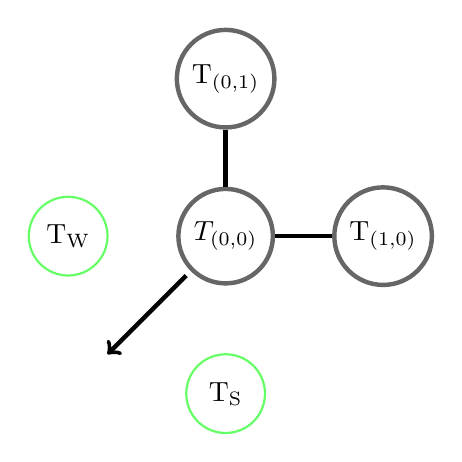
\begin{tikzpicture}[
roundnode/.style={circle, draw=black!60, ultra thick,  minimum size=10mm},
ghostnode/.style={circle, draw=green!60, thick, minimum size = 10mm},
]
\node[roundnode] (center) {$T_{(0,0)}$};
\node[ghostnode] (left) [left of=center] {T$_\text{W}$};
\node[roundnode] (right) [right of=center] {T$_{(1,0)}$};
\node[roundnode] (above) [above of=center] {T$_{(0,1)}$};
\node[ghostnode] (below) [below of=center] {T$_\text{S}$};


\draw[ultra thick,-] (above.south) -- (center.north);
\draw[ultra thick,-] (right.west) -- (center.east);
\draw[ultra thick,->] (-0.5,-0.5) -- (-1.5,-1.5);

\end{tikzpicture}
\end{center}
As a normalised vector, it will be 
\begin{center}
    $\hat{\textbf{n}} = \frac{1}{\sqrt{2}}(-1,-1)^T$.
\end{center}
We can use this in our boundary condition to create a first order difference approximation for $T_W + T_S$.
\begin{center}
  \[\bigg{(}\frac{\partial T}{\partial x},\frac{\partial T}{\partial y}\bigg{)}\cdot \frac{1}{\sqrt{2}}(-1,-1)^T = 0\]
  \[\bigg{(}\frac{\partial T}{\partial x},\frac{\partial T}{\partial y}\bigg{)}\cdot (-1,-1)^T = 0\]
  \[\bigg{(}\frac{\partial T}{\partial x}+\frac{\partial T}{\partial y}\bigg{)} = 0\]
  \[\frac{T-T_W}{0.01}+\frac{T-T_S}{0.01} = 0\]
  \[T_W+T_S=2T.\]
\end{center}
Substituting this into our stencil, we can see that 
\begin{center}
\[4T_{(0,0)}-T_{(0,1)}-T_{(1,0)}-T_{W}-T{S}=0\]
\[4T_{(0,0)}-T_{(0,1)}-T_{(1,0)}-2T_{(0,0)}=0\]
\[2T_{(0,0)}-T_{(0,1)}-T_{(1,0)}=0.\]
\end{center}

\paragraph*{Nodes E-D:} On the nodes E-D, the normal unit vector will face directly south. 
\begin{center}
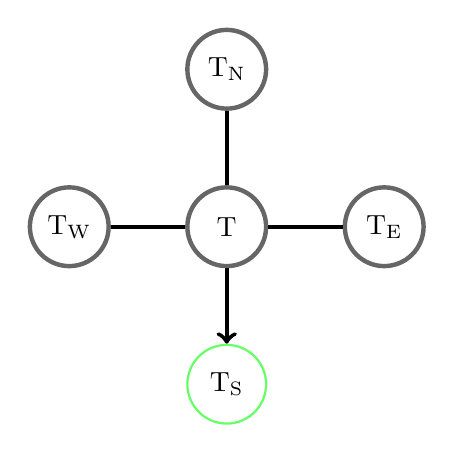
\begin{tikzpicture}[
roundnode/.style={circle, draw=black!60, ultra thick,  minimum size=10mm},
ghostnode/.style={circle, draw=green!60, thick, minimum size = 10mm},
]
\node[roundnode] (center) {T};
\node[roundnode] (left) [left of=center] {T$_\text{W}$};
\node[roundnode] (right) [right of=center] {T$_\text{E}$};
\node[roundnode] (above) [above of=center] {T$_\text{N}$};
\node[ghostnode] (below) [below of=center] {T$_\text{S}$};

\draw[ultra thick,-] (left.east) -- (center.west);
\draw[ultra thick,-] (above.south) -- (center.north);
\draw[ultra thick,-] (right.west) -- (center.east);
\draw[ultra thick,<-] (below.north) -- (center.south);
\end{tikzpicture}
\end{center}
This can be written as 
\begin{center}
  $\hat{\textbf{n}}=(0,-1)^T$.
\end{center}
Using the same boundary rule for the edge A-E-D (which contains the edge E-D) we can find a first order forward difference for $T_S$.
\begin{center}
\[\bigg{(}\frac{\partial T}{\partial x},\frac{\partial T}{\partial y}\bigg{)}\cdot (0,-1)^T = 0\]
\[-\frac{\partial T}{\partial y}=0\]
\[\frac{T-T_S}{0.01}=0\]
\[T_S=T\]
\end{center} 
Using this in our finite difference equation, we get the following equation for a node along the boundary E-D.
\begin{center}
  \[4T-T_S-T_N-T_W-T_E=0\]
  \[4T-T-T_N-T_W-T_E=0\]
  \[3T-T_N-T_W-T_E=0.\]
\end{center}
As an example, let us look at node $T_{(3,0)}$.
\begin{center}
  $3T_{(3,0)}-T_{(3,1)}-T_{(2,0)}-T_{(4,0)}=0$.
\end{center}
Each other node along the boundary will be similar to this node.
\subsubsection{Boundary B-C}
There are three nodes that we care about on the boundary B-C. The boundary condition along these nodes are
\[k\boldsymbol{\nabla}T\cdot\hat{\textbf{n}} = h(T_{\infty} - T)\]
where $k=3\text{Wm}^{-1}\text{C}^{-1}, h=20\text{Wm}^{-2}\text{C}^{-1}, T_\infty=20$.


\begin{center}
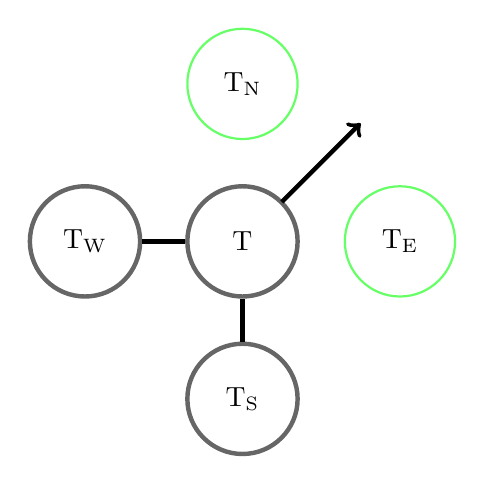
\begin{tikzpicture}[
roundnode/.style={circle, draw=black!60, ultra thick,  minimum size=14mm},
ghostnode/.style={circle, draw=green!60, thick, minimum size = 14mm},
]
\node[roundnode] (center) {T};
\node[roundnode] (left) [left of=center] {T$_\text{W}$};
\node[ghostnode] (right) [right of=center] {T$_\text{E}$};
\node[ghostnode] (above) [above of=center] {T$_\text{N}$};
\node[roundnode] (below) [below of=center] {T$_\text{S}$};

\draw[ultra thick,-] (left.east) -- (center.west);
\draw[ultra thick,->] (0.5,0.5) -- (1.5,1.5);
\draw[ultra thick,-] (below.north) -- (center.south);
\end{tikzpicture}
\end{center}
The unit normal on each node will be facing directly north-east as the boundary is diagonal. Therefore
\[\hat{\textbf{n}} = \frac{1}{\sqrt{2}}(1,1)^T.\]
Using this in our boundary condition (along with leaving the ambient temperature as a variable) yields
\[3\bigg{(}\frac{\partial T}{\partial x},\frac{\partial T}{\partial y}\bigg{)}\cdot\frac{1}{\sqrt{2}}\big{(}1,1\big{)}^T=20\big{(}T_\infty-T\big{)}\]
Using first order forward differences for $\frac{\partial T}{\partial x}$ and $\frac{\partial T}{\partial y}$ and rearranging to solve for $\text{T}_\text{N}+\text{T}_\text{E}$
\[\frac{3}{\sqrt{2}}\bigg(\frac{T_E-T}{0.01}+\frac{T_N-T}{0.01}\bigg)=20T_\infty-20T\]
\[T_E+T_N-2T=\frac{\sqrt{2}}{3}\big(0.2T_\infty-0.2T\big)\]
\[T_E+T_N=\frac{0.2T_\infty\sqrt{2}}{3}+\frac{6-0.2\sqrt{2}}{3}T.\]
For two of the nodes along the B-C boundary, either $T_E$ or $T_N$ will be constant. This results in all nodes along the border having the following equation for their rate of change
\[\bigg(2+\frac{0.2\sqrt{2}}{3}\bigg)\text{T}-\text{T}_{S}-\text{T}_{W} =\frac{0.2T_\infty\sqrt{2}}{3}\]
 
\subsection{Node Ordering}
One last thing we must do is construct a mapping from the 2D array of nodes to a 1D array of nodes. This is useful when creating the vectors $x$ and $b$ in the linear equation $Ax=b$.
\\\\
Because we have a $6 \times 6$ array (ignoring the missing or null nodes in the top right corner) we can transform this into a 1D array with 36 values. We can use the following assumptions to construct the map \begin{itemize}
\item Our index is $(i,j)$ with $i$ being the horizontal coordinate and $j$ being the vertical coordinate 
\item (0,0) is the bottom left node 
\item ($i+1$, $j$) is to the right of ($i$,$j$) and ($i$,$j+1$) is above ($i$, $j$)
\end{itemize}
From this we can deduce that every time we move across the 2D array, we are moving 1 unit across in the 1D array, and every time we move up in the 2D array, we are moving 6 across in the 1D array. Therefore,
\begin{center}
$(i,j) \to i+6j$.
\end{center}
For example, the equation
\[2T_{(0,0)}-T_{(1,0)}-T_{(0,1)}=0\]
will transform into
\[2T_0-T_1-T_6=0.\]
\subsection{Matrix Construction}
Using our node ordering, we can write out all the equations in a certain ordering (See Appendix A1). This can then be rewritten as a linear system, $Ax=b$, where $A$ is the coefficient matrix of the equations, $x$ is the unknown temperature values and b is the right hand side values of the equations.\\\\Using the spy() command on $A$, we can see that it has a banded structure, noting that it has a total bandwidth of 13.
\begin{figure}[H]
	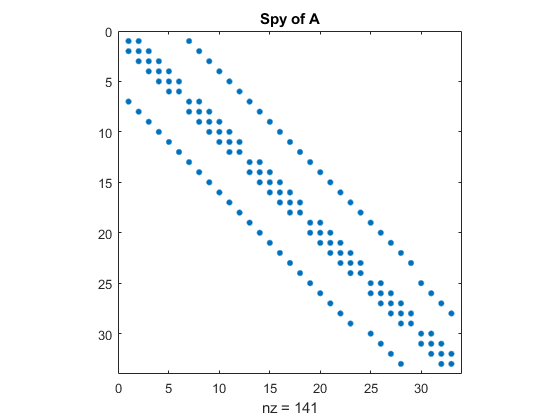
\includegraphics[width=\linewidth]{images/spyA.png}
	\caption{Spy of $A$.}
	\label{fig:spyA}
\end{figure}
\subsection{Checking SPD}
The matrix $A$ is both symmetric and positive definite. This can be verified with Matlab.\\If $A$ is symmetric, then for all $(i, j)\in$ dim$(A), A(i, j) = A(j, i)$. To check that it is symmetric, the matrix minus its transpose can be plotted. If all the values are zero, then it is symmetric.
\begin{figure}[H]
	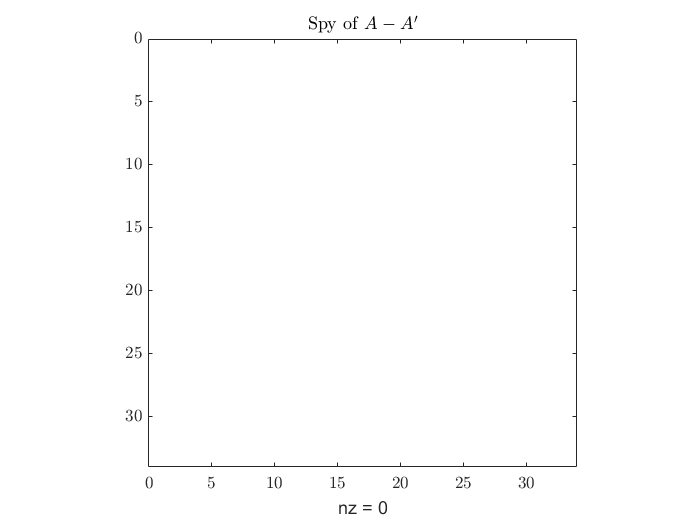
\includegraphics[width=\linewidth]{images/spySymmetric.png}
	\caption{Spy of $A-A'$.}
	\label{fig:spySymmetric}
\end{figure}
The spy command produces a plot graph with plots in coordinates where the value of the matrix (at the same coordinate) is not zero. Since the figure produced by the spy command has no plots, every value in the matrix A-A' is zero, which implies that A is symmetric.
\\\\To show that A is positive definite, it is enough to show that the eigenvalues are all positive. Plotting the values of the eigenvalues along an axis representing the $n^{th}$ eigenvalue yields\begin{figure}[H]
	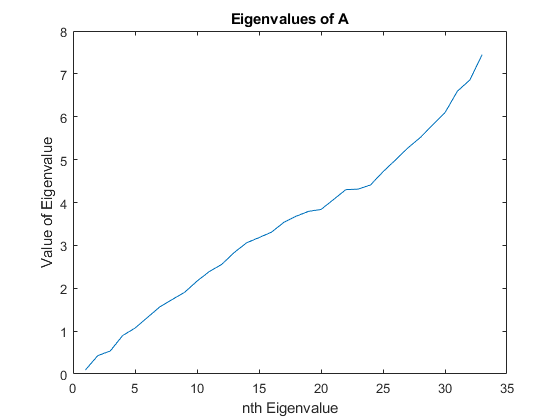
\includegraphics[width=\linewidth]{images/eigenvaluePlot.png}
	\caption{Eigenvalues of $A$.}
	\label{fig:eigenvalues}
\end{figure}

\section{Storage and Solutions}
In this section, direct and iterative methods are used to solve for the vector $x$, such that:
\[Ax=b\]
This vector will be the approximate final temperatures at the discrete points along the electronic component. \\\\Other factors will also be briefly mentioned, including fill-in, storage size, run time, flop count and residual norms.\\\\Fill-in is the number of zero elements that become non-zero when the matrix is changed (in this case, it will be when Cholesky factorisation is performed in the Direct Methods).
\subsection{Direct Methods}
Direct methods involve directly solving for the vector x by factorsing the matrix A and performing forward and backward substitution.
\subsubsection{Full Storage}
The Full Storage solution is very simple. Because we have a linear system, we can just factorise the matrix into an upper and lower system, then perform forward and backward substitution to solve for the steady-state heat distribution. Because our coefficent matrix is symmetric positive definite, Cholesky factorisation can be used to factorise the coefficient matrix. Comparing the original matrix and the factorised matrix side by side, the fill-in can be found.
\begin{figure}[H]
	\hspace{-8mm}
	\begin{subfigure}[b]{0.6\textwidth}
		\hspace{-8mm}
		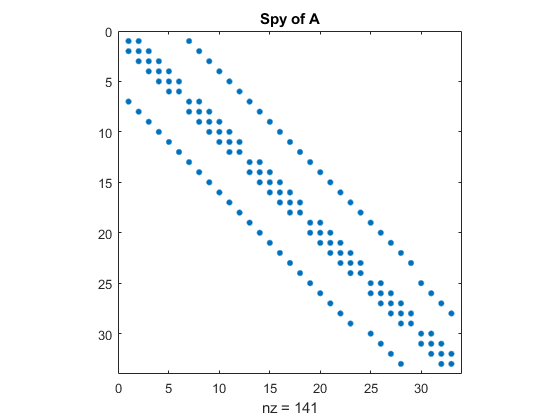
\includegraphics[width=\textwidth]{images/spyA.png}
	\end{subfigure}
	\hspace{-8mm}
	\begin{subfigure}[b]{0.6\textwidth}
		\hspace{-8mm}
		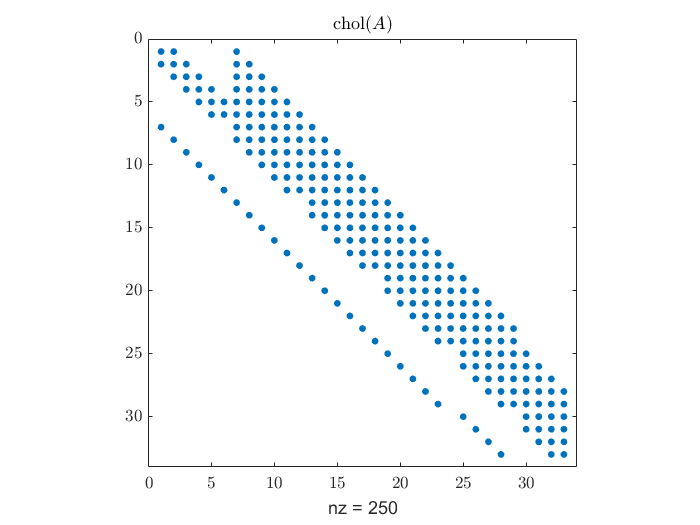
\includegraphics[width=\textwidth]{images/cholA.png}
	\end{subfigure}
\end{figure}
By analysing the number of non-zero elements, it can be seen that the fill-in from using the Cholesky algorithm is 109.
\subsubsection{Packed Storage}
The packed storage is a linear direct method solution. That because we just need to factorise the matrix into upper system. In addition, as the coefficients of the matrix is SPD, then we can use Cholesky factorisation. Therefore, we are able to reduce the size of the matrix into a array a, where the array a is the number of elements in the matrix being store in only one vector. To implement Cholesky factorisation by using packed storage structure, it is necessary that to convert the two-dimension matrix into one dimensional vector. How can we convert this? The answer is by using mapping technique which is as follow:
\\
$A(i,j) \to a(i+j(j-1)/2)$. 
\\
After applying this mapping technique Cholesky algorithm will give us the solution of the steady-state heat distribution. 

\subsubsection{Band Storage}
A banded system is a matrix where all non-zero elements are within a certain distance of the main diagonal (which depends on the matrix). The matrix looked at previously is a banded system, however, it is not ordered in an efficient manner, as the fill-in is unnecessarily increased due to the number of 0-diagonals between the inner tridiagonal and the outer diagonals. \\\\Using a technique called RCM ordering, the average bandwidth can be reduced, along with the level of fill in when Cholesky factorisation is performed. The b vector is also reordered using the same reordering vector to keep the equation $Ax=b$ equivalent. The reordered A matrix using RCM ordering and the banded matrix B will look like
\begin{figure}[H]
	\hspace{-8mm}
	\begin{subfigure}[b]{0.79\textwidth}
		\hspace{-8mm}
		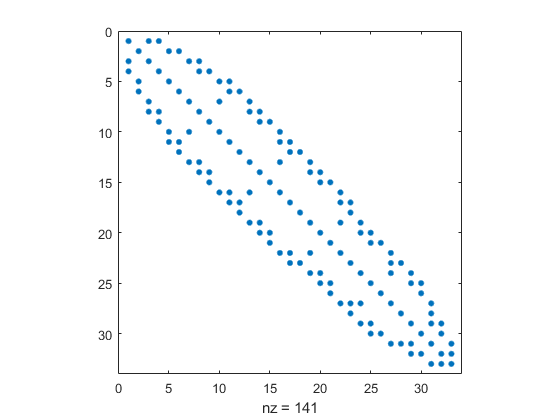
\includegraphics[width=\textwidth]{images/ARCM.png}
	\end{subfigure}
	\hspace{-10mm}
	\begin{subfigure}[b]{0.21\textwidth}
		\hspace{-10mm}
		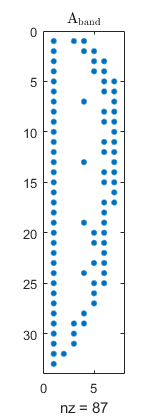
\includegraphics[width=\textwidth]{images/band.png}
	\end{subfigure}
\end{figure}
The next step is to convert the RCM ordering to a banded storage matrix, denoted $B$. Because $A$ is symmetric, we can get away with only storing the upper or lower part of the matrix. The dimensions of this matrix are $\mathbb{R}^{n\times p}$, where n is the row or column count of $A$, and p is the upper bandwidth of $A$. To change the storage, we must create a new mapping from the elements of the upper portion of $A$ to $B$.
\begin{align*}
A(i,j)\to B(i,j-i+1), \text{ where } i,j < \text{dim}(A).
\end{align*}
To perform Cholesky factorisation on this matrix, and keeping the factorised matrix in the same dimension, the regular Cholesky factorisation method can be retooled using the previously mentioned mapping for band storage.
The new algorithm must now check that the index $j-i+1$ is within the width of the matrix, as the column is less than the row count, and trying to access $A(i,j-i+1)$ would result in an error if $j-i+1$ was greater than the number of columns. In the original matrix, these values would have just been 0, and no change would happen.\\\\Performing the Banded Cholesky algorithm on the banded matrix yields
\begin{figure}[H]
	\begin{center}
		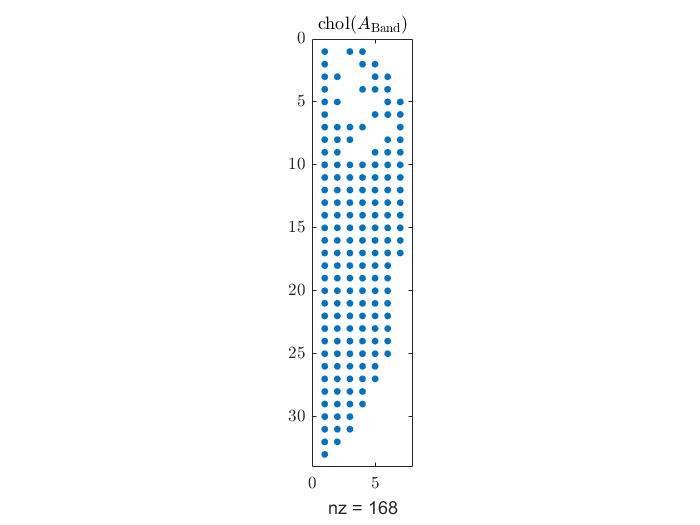
\includegraphics[width=\linewidth]{images/cholband.png}
		\caption{Spy of Banded $A$ after the Cholesky factorisation.}
		\label{fig:cholband}
	\end{center}
\end{figure}
It can be seen that the fill-in of this storage method is 81.\\To use this factorised matrix, a new forward and backward method must be constructed. Luckily, the previous mapping can still be used. Care must be taken when working in a non-square matrix in both forward and backward substitution, as it is still possible to access elements outside of the new array. Adding checks before accessing the array to make sure the given index is within the bounds of the array solves the problem, as any element outside of the array would just be zero, and performing no operation results in the same outcome. The mapping is also substituted into the forward and backward substitution algorithms.\\\\Solving the system of equations using the new forward and backward substitution, the following heatmap of the component is obtained.
\begin{figure}[H]
	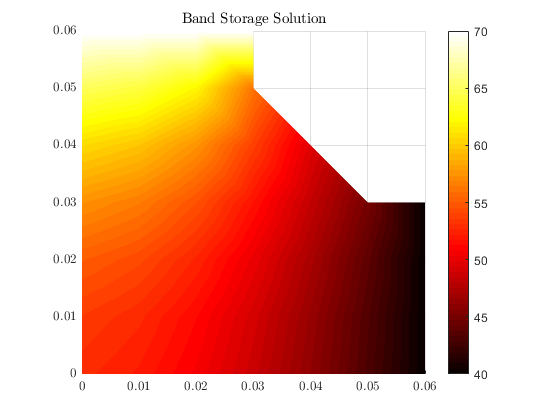
\includegraphics[width=\linewidth]{images/bandsolution.png}
	\caption{Solution using Band Storage.}
	\label{fig:bandsolution}
\end{figure}
\subsubsection{Sparse Storage}
A sparse system is a matrix that has no structure to where the non-zero elements appear, but still has a large number of zero values. To pre-emptively reduce the fill-in from the Cholesky factorisation, Approximate Minimum Degree (AMD) is used to reorder the A matrix. An AMD permutation will change the ordering of the matrix such that it has when Cholesky factorisation is performed, many of the zero values will stay zero. This reduces storage space when the new factorised matrix is stored using sparse storage, and can reduce runtime when implemented properly. In this case, sparse storage was only used to demonstrate storage benefits.\\\\Using matlab's inbuilt \textbf{symamd} function, the following matrix is obtained
\begin{figure}[H]
	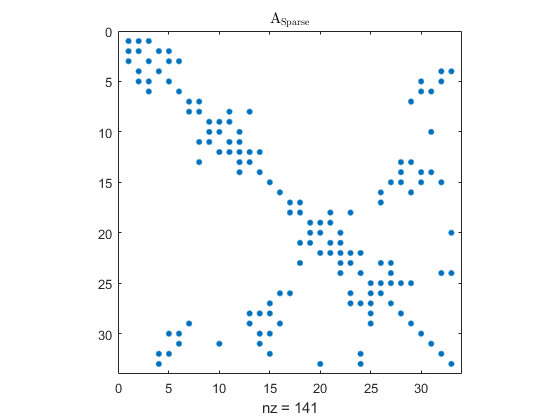
\includegraphics[width=\linewidth]{images/A_SPARSE.png}
	\caption{Spy of $A$ Sparse.}
	\label{fig:A_SPARSE}
\end{figure}
This can be stored in sparse storage using Matlab's \textbf{sparse} function. The size of the sparse matrix is only 2528 bytes, nearly 3.5 times smaller. The Cholesky algorithm is changed to check if any value at the index it accesses is 0 and if it is, it skips performing the operation involving that index. This reduces the flop count of the algorithm, but increases computation time due to if statements being inefficient when accessing a sparse matrix on Matlab. Viewing the AMD ordered factorised matrix, it can be seen that the fill-in is fairly small.
\begin{figure}[H]
	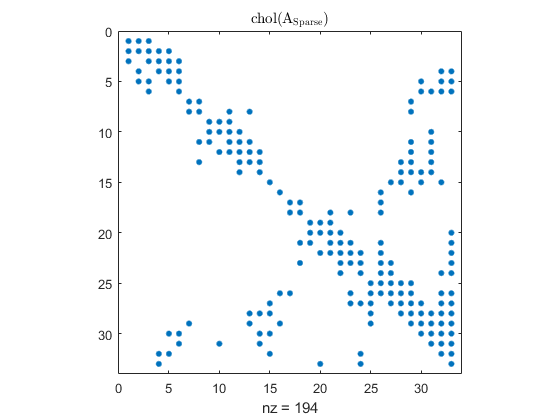
\includegraphics[width=\linewidth]{images/A_SPARSE_CHOL.png}
	\caption{Spy of $A$ Sparse after Cholesky factorisation.}
	\label{fig:A_SPARSE_CHOL}
\end{figure}
Looking at the difference in the number of non-zero elements, it can be seen that the fill in using AMD ordering is 53. The final heatmap is
\begin{figure}[H]
	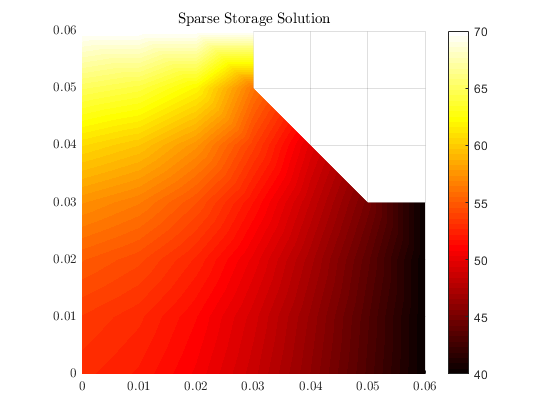
\includegraphics[width=\linewidth]{images/sparsestorage.png}
	\caption{Sparse Solution.}
	\label{fig:sparsestorage}
\end{figure}

\subsection{Iterative Methods and Compressed Sparse Row Format Storage}
Iterative methods involve solving for the vector x by guessing an initial value for x, then updating it using the formula
\[x^{k+1}=Tx^k+c\]
where T is the iteration matrix. This iteration matrix depends on which method is used.\\\textbf{Compressed sparse row format} (CSR), stores all the non-zero elements that are in a given matrix and it's respected row and column indices of these non-zero elements. CSR consists of three arrays: \textbf{rb} which stores the index of where each new row begins in both \textbf{c} and \textbf{v}; \textbf{c} which consists of the column indices; and \textbf{v} which contains the value of these elements. $\textbf{rb}$ ends with $nz + 1$, where $nz$ is the total number of non-zero elements in $A$.
\\\\
CSR storage was used to store $A$. The iterative methods: Jacobi, Gauss-Seidel, Successive Over-relaxation (SOR), Conjugate Gradient Methods were used to solve for $x$ given that $Ax = b$. Unlike the direct methods used for the previous storages of $A$, iterative methods do not require the matrix to be factorised or modified. The idea behind iterative methods is to gradually approach an approximation to the exact solution. The stationary iterative methods, Jacobi, Gauss-Seidel, and SOR are all based on the splitting of $\textbf{A} = \textbf{D} + \textbf{L} + \textbf{U}$.
\\\\
To change the storage of $A$ using CSR storage, the matrix had to first be sorted into three vectors $\textbf{r}$, $\textbf{c}$, and $\textbf{v}$, where $\textbf{r}$ was the row indices. This was computed using Matlab's built in function \textbf{find}. This function returns $\textbf{r}$, $\textbf{c}$, and $\textbf{v}$ where the column indices are in ascending order. Therefore, $\textbf{r}$ must be ordered so the row indices are in ascending order and $\textbf{c}$, and $\textbf{v}$ needed to be reordered to correctly represent $A$. Then, $\textbf{r}$ must to be converted to $\textbf{rb}$. 
\\\\
As $A$ has now been converted to $\textbf{rb}$, $\textbf{c}$, and $\textbf{v}$ the iterative methods must be altered to account for this change. When $A$ is multiplied by $x$ throughout the iterative methods, the method for solving $Ax$ had to be altered. This ultimately removed the unnecessary multiplications as all the zero elements had been removed. This should result in the iterative methods running faster than they would if the A matrix had been stored using Full Storage.

\subsubsection{The Jacobi Method}
The first iterative method that is used to solve for $x$ using CSR storage is the \textbf{Jacobi method}.
\\\\
The Jacobi Method is:
\\\\
$$x_{i}^{(k+1)} = \frac{1}{a_{ii}}(b_i-{\sum_{j=1}^{i-1}}_{j\neq i}a_{ij}x_{j}^{(k+1)}, i = 1, 2, ..., n$$
\\\\
As mentioned above, the Jacobi method function had to be altered as $A$ was stored in CSR storage. The three vectors then had to be integrated in the function. 
\begin{figure}[H]
	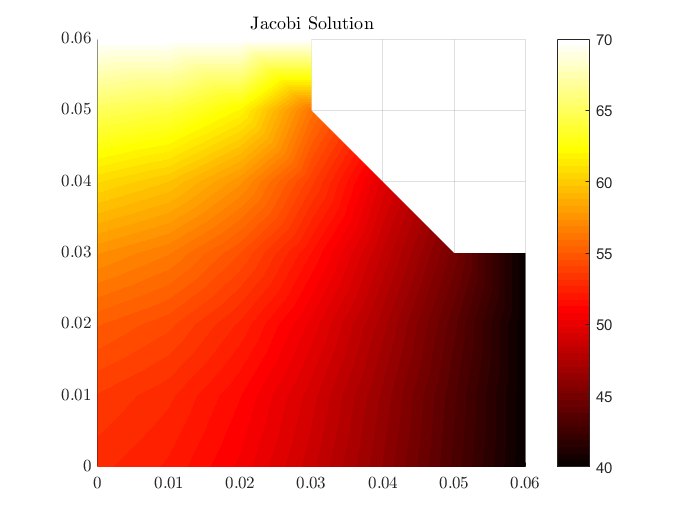
\includegraphics[width=\linewidth]{images/jacobisolution.png}
	\caption{Jacobi Solution.}
	\label{fig:jacobi}
\end{figure}

\subsubsection{The Gauss-Seidel Method}
The second iterative method that is used to solve for $x$ using CSR storage is the Gauss-Seidel method.
\\\\
The Gauss-Seidel Method is:
\\\\
$$x_{i}^{(k+1)} = \frac{1}{a_{ii}}(b_i-\sum_{j=1}^{i-1}a_{ij}x_{j}^{(k+1)}-\sum_{j=i+1}^{n}a_{ij}x_{j}^{(k)}), i = 1, 2, ..., n$$
\\\\
The Gauss-Seidel function also had to be altered to account for the different storage. 

\begin{figure}[H]
	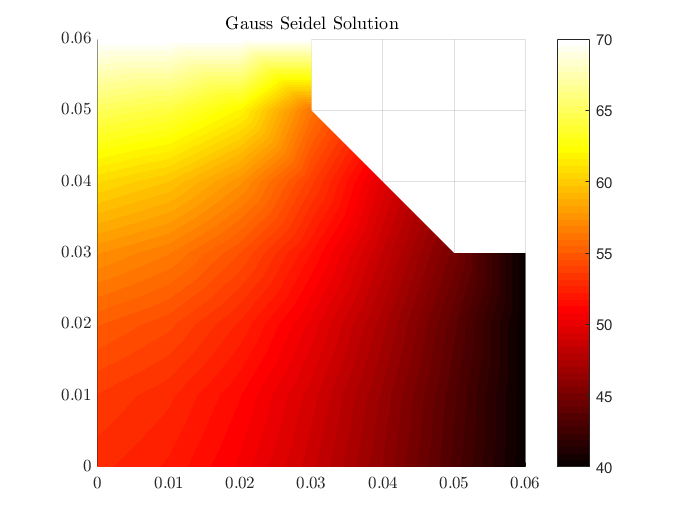
\includegraphics[width=\linewidth]{images/gaussseidelsolution.png}
	\caption{Gauss-Seidel Solution.}
	\label{fig:gauss}
\end{figure}

\subsubsection{The Successive Over-relaxation Method}
The third iterative method that is used to solve for $x$ using CSR storage is the Successive Over-relaxation (SOR) method. The SOR method has much faster convergence than Jacobi and Gauss-Seidel method, provided the $\omega$ selected is the optimal value. This is because SOR is designed so that $\omega$ minimises the spectral radius $\rho(T_{SOR})$. For solving this solution, the formula for finding the optimal $\omega$ was used as the $\omega$ value.
\\\\
$\omega_{opt} = \frac{2}{1+\sqrt{1-\rho(T_{J})^{2}}}$.
\\\\
The SOR Method is: 
\\\\
$$x_{i}^{(k+1)} = (1-\omega)x_{i}^{(k)}+\frac{\omega}{a_{ii}}(b_i-\sum_{j=1}^{i-1}a_{ij}x_{j}^{(k+1)}-\sum_{j=i+1}^{n}a_{ij}x_{j}^{(k)}), i = 1, 2, ..., n$$
\\\\
The SOR function was also altered to account for the change in storage.

\begin{figure}[H]
	\includegraphics[width=\linewidth]{images/sorsolution.png}
	\caption{SOR Solution.}
	\label{fig:sor}
\end{figure}

\subsubsection{The Conjugate Gradient Method}
The fourth iterative method that is used to solve for $x$ using CSR storage is the Conjugate Gradient method. If the coefficient matrix is symmetric positive definite, the Conjugate Gradient method is very powerful.
\\\\
\textbf{Algorithm for Conjugate Gradient Method}
\begin{center}
$\textbf{r}^{(0)}=\textbf{b-Ax}^{(0)}, \textbf{d}^{(0)}=\textbf{r}^{(0)}$.
\end{center}
\begin{enumerate}
\item $\alpha_{k} = (\textbf{r}^{(k)^{T}}\textbf{r}^{(k)})/(\textbf{d}^{(k)^{T}}\textbf{Ad}^{(k)})$
\item $\textbf{x}^{(k+1)}=\textbf{x}^{(k)}+\alpha_{k}\textbf{d}^{(k)}$
\item $\textbf{r}^{(k+1)}=\textbf{r}^{(k)}-\alpha_{k}\textbf{Ad}^{(k)}$
\item $\beta_{k} = (\textbf{r}^{(k+1)^{T}}\textbf{r}^{(k+1)})/\textbf{r}^{(k)^{T}}\textbf{r}^{(k)}$
\item $\textbf{d}^{(k+1)}=\textbf{r}^{(k+1)}+\beta_{k}\textbf{d}^{(k)}$
\end{enumerate}

\begin{figure}[H]
	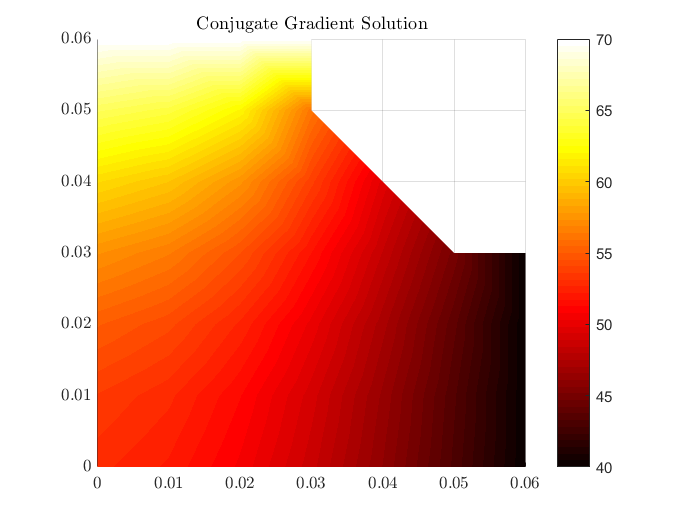
\includegraphics[width=\linewidth]{images/conjugategradientsolution.png}
	\caption{Conjugate Gradient Solution.}
	\label{fig:conjugate}
\end{figure}

\section{Efficiency Comparison}
The following section investigates which numerical method or methods provide the greatest efficiency in solving problems similar to the electronic component. This involves the storage size of the coefficient matrix and the time it takes to find the solution for each method.

\subsection{Bandwidth and Level of Fill-in for each different Node Ordering}
Because memory is a key concern when working with large data structures, it is important to choose a method that reduces the storage size. The bandwidth and fill-in are both components that determine how much memory the factorised matrix will take up. Fill-in is the number of zero elements in the matrix that turn into non-zero elements after factorisation is completed. 

\subsection{Memory (for Direct Methods)}
Memory for the $A$ that were used to solve $x$ using direct methods was compared to see which storage required the least memory.
\begin{center}
\begin{tabular}{c c c c c}
Name & Size & Bytes & Class & Attributes \\
\hline
$A$ & $33 \times 33$ & $8712$ & double & \\
$A$ Banded Storage & $33 \times 7$ & $1848$ & double & \\
$A$ Packed Storage & $1 \times 561$ & $4488$ & double & \\
$A$ Sparse Storage & $33 \times 33$ & $2528$ & double & sparse \\
\end{tabular}
\end{center}
\begin{figure}[H]
	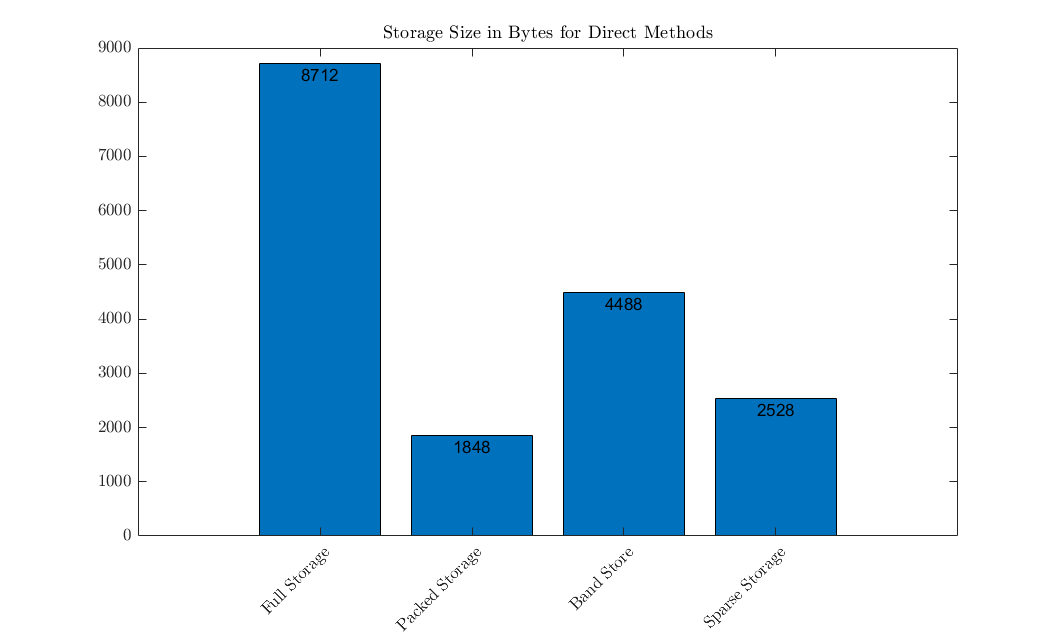
\includegraphics[width=\linewidth]{images/MemoryGraph.png}
	\caption{Size in bytes for storage size for each direct method.}
	\label{fig:memory}
\end{figure}
Full Storage was found to require the most memory (8712 Bytes), whereas Band storage was found to require the least amount of memory (1848) of the Direct Methods. This is because the bandwidth of the matrix is rather small at this scale, and it only stores values from the inner diagonal to the outer diagonal. However, if the mesh was to be made finer, it may end up less efficient than the sparse storage method. Sparse storage scales more efficiently as the mesh becomes finer, as the number of non-zero elements in each row and column does not increase. 

\subsection{Iterations (for Iterative Methods)}
The efficiency of iterative approaches depends on the accuracy desired for the solution. Each method needs to converge to an answer within a tolerance. The SOR method also relies on a value $\omega$ to start with in order to converge faster than other methods. The tolerance was $1\times10^{-5}$ and the $\omega$ was the optimal $\omega$ for this $A$ matrix.
\\\\
The number of iterations for each iterative method (Jacobi, Gauss-Seidel, SOR, and Conjugate Gradient method) were recorded and graphed.
\begin{figure}[H]
	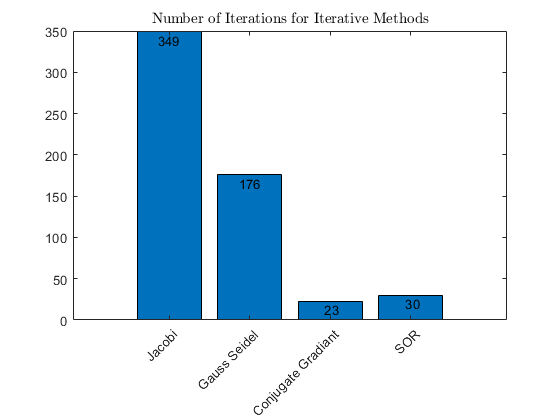
\includegraphics[width=\linewidth]{images/IterationsGraph.png}
	\caption{Number of Iterations for each Iterative Method}
	\label{fig:iterations}
\end{figure} 
The Jacobi method required the most iterations to converge, followed by Gauss-Seidel, SOR, then Conjugate Gradient method.
\begin{figure}[H]
	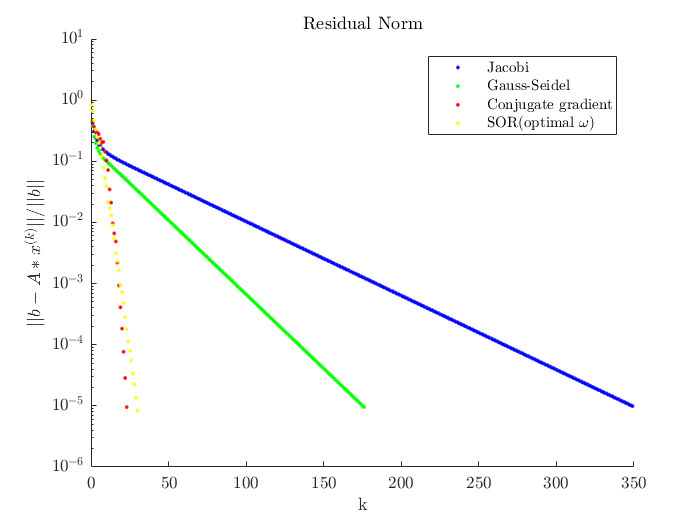
\includegraphics[width=\linewidth]{images/ResidualNormGraph.png}
	\caption{Residual Norm for each Iterative Methods}
	\label{fig:res}
\end{figure}

\subsection{Runtime (Direct and Iterative)}
The runtime for solving $x$ using each type of storage was recorded using Matlab's built in functionality (tic and toc). The runtime was recorded between the time taken to solve for $x$ with the storage for $A$ already calculated. Calculations, for example, $\omega_{opt}$ were not counted towards the runtime. Cholesky factorisation, forward substitution, backwards substitution, Jacobi method, Gauss-Seidel method, SOR method, and Conjugate Gradient Method were the only calculations counted towards the runtime.
\\\\
The calculations for each storage was run $1000$ times each then averaged out to get a more accurate representation of the runtime.
\begin{figure}[H]
	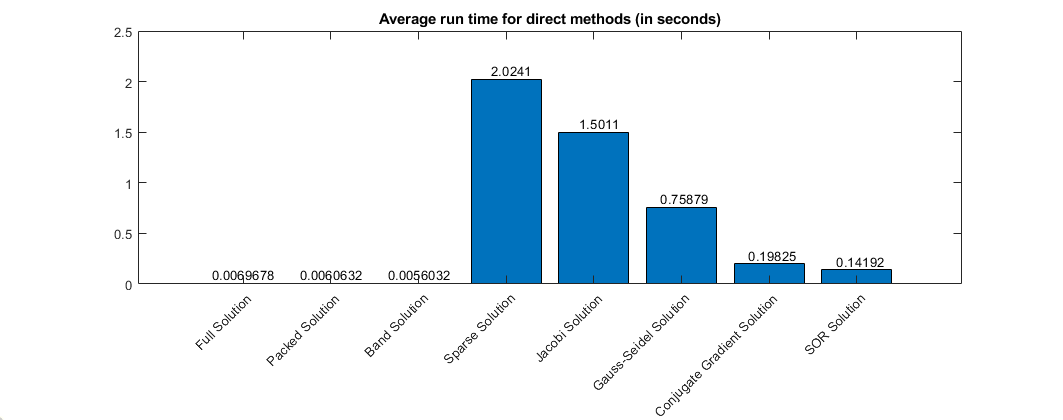
\includegraphics[width=\linewidth]{images/RuntimeGraph.png}
	\caption{Runtime for solving each of the Direct and Iterative Methods.}
	\label{fig:runtime}
\end{figure}
Figure \ref{fig:runtime} clearly shows that the iterative methods generally took the longest to execute, with the exception of the Sparse Solution. Sparse storage took longer to factorise using Cholesky compared to the other storages using Cholesky as the if statements are inefficient in the algorithm.
\\\\
Banded Storage took the least amount of time to run on average, however if the sparse structure was accessed better, it would be much more competitive with the other direct methods.

\subsection{Floating Point Operations (Direct and Iterative)}
\textbf{Floating point operation count} (flop count) is referred to as the number of arithmetic operations performed by an algorithm during its execution. For the direct and iterative methods, the flop count was calculated for every multiplication and addition. A flop was counted for every multiplication and addition in the nested for loops. However, this is only an estimation as some of the multiplications are performing more than one flop, but are only counted as one.
\begin{figure}[H]
	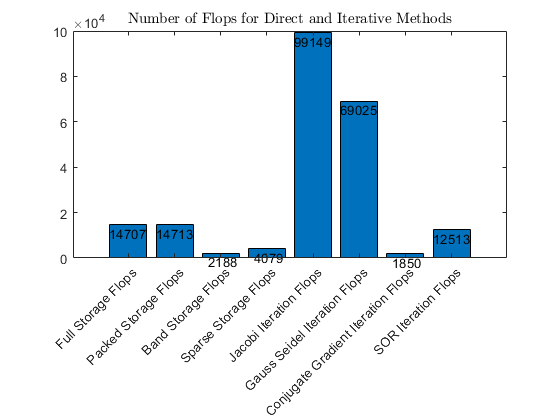
\includegraphics[width=\linewidth]{images/FlopsGraph.png}
	\caption{Flops for each Direct and Iterative Methods.}
	\label{fig:flops}
\end{figure}
The Jacobi method was found to contain the most flops, whereas the Conjugate Gradient method was found to have the least flops. Interestingly, the Cholesky factorisation, forward and backwards substitution for Full and Packed Storage had approximately the same amount of flops, but Band and Sparse storage had significantly less than the other Cholesky factorisation. The packed and full had approximately $5.25$ times more flops than the band and sparse.

\subsection{Tolerance Required for Iterative Methods)}
The following discusses the tolerance that is required for the iterative methods to produce a solution that is visually indistinguishable from that produced by the direct method. The tolerances: $1\times10^{-10}, 1\times10^{-5}, 1\times10^{-3}, 2\times10^{-3}, 1\times10^{-2}, 1\times10^{-1}, 0.5, 1$ were compared against the exact solution for each iterative method.
\\\\
It was found that for the Jacobi Method, SOR Method, Gauss Method that $1\times10^{-5}$ was the tolerance where the solution was visually indistinguishable. However, for the Conjugate Gradient Method the tolerance was $2\times10^{-3}$ where the solution was visually indistinguishable.
\section{Effect of Ambient Temperature} 
The electronic component will only function if the temperature at the point (0.03, 0.03) is within $50-55\degree$C. This temperature could change depending on what the ambient air temperature is. Earlier in the model, we have assumed that this temperature is $20\degree$C. To find the affect of different ambient temperatures, we can run the model through a loop, changing the values of the ambient temperature from $0\degree$C to $60\degree$C in increments of $0.01\degree$C. Printing a value of the ambient temperature and the inner component temperature when the inner component temperature is within a tolerance of $0.001\degree$C, we can find rough estimates of the lower and upper bounds of the ambient temperature. These are found to be 
\[\text{Lower bound }\approx 1.72\degree\text{C},\]
\[\text{Upper bound }= 55\degree\text{C}.\]
The algorithm can then be refined to search finer values around the lower bound. Searching within a tolerance of $10^{-6}$, the ambient temperature comes out to approximately 1.727406$\degree$C. As this is a very specific temperature, and the real world is not perfect, we can think of the lower bound as just being $2\degree$C. The heat distributions at the lower and upper bounds are \begin{figure}[H]

	\begin{subfigure}[b]{0.49\textwidth}
		\hspace{-8mm}
		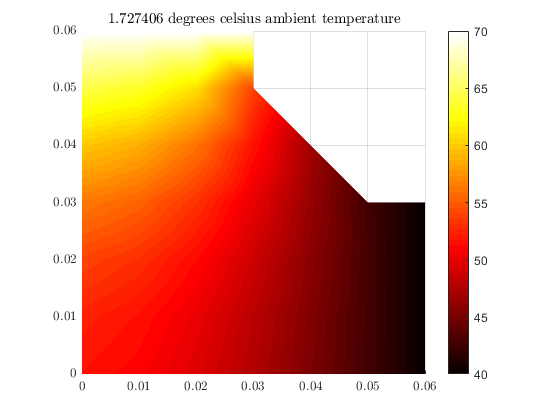
\includegraphics[width=\textwidth]{images/coldplate.png}
	\end{subfigure}
	\hspace{-8mm}
	\begin{subfigure}[b]{0.49\textwidth}
		\hspace{-8mm}
		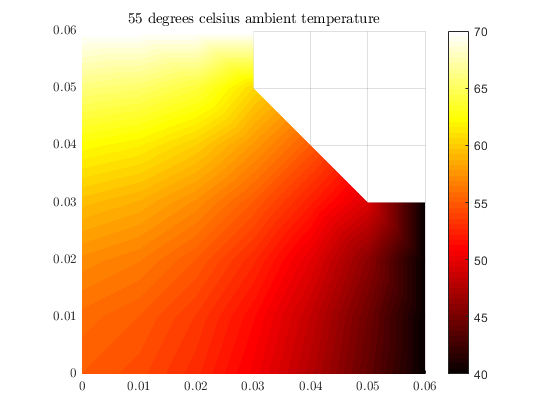
\includegraphics[width=\textwidth]{images/hotplate.png}
	\end{subfigure}
\end{figure}
We recommend that the component only be deployed in locations with a temperature that never goes below $2\degree$C or above $55\degree$C.
\section{Recommendations}
The following section is recommendations for the component or for components similar to the one discussed in this report.
\subsection{Distribution of the Component}
The heat distribution of the component fans smoothly from 70$\degree$C at the upper boundary to 40$\degree$C on the right boundary. The ambient temperature is an important factor that affects the distribution of the heat on the component. As discussed in section 5, the range of ambient temperatures this component can safely operate
in is between 2$\degree$C and 55$\degree$C, such that the temperature at the point (0.03, 0.03) remains between 50 and 55$\degree$C. The lower ambient temperature causes the heat at the 70$\degree$C boundary to drop off much faster. 
\\\\
A map of the world's yearly average temperatures show that the component should not be deployed in countries near the north pole, along with Antarctica, and high altitude countries. 
\begin{figure}[H]
	\center
	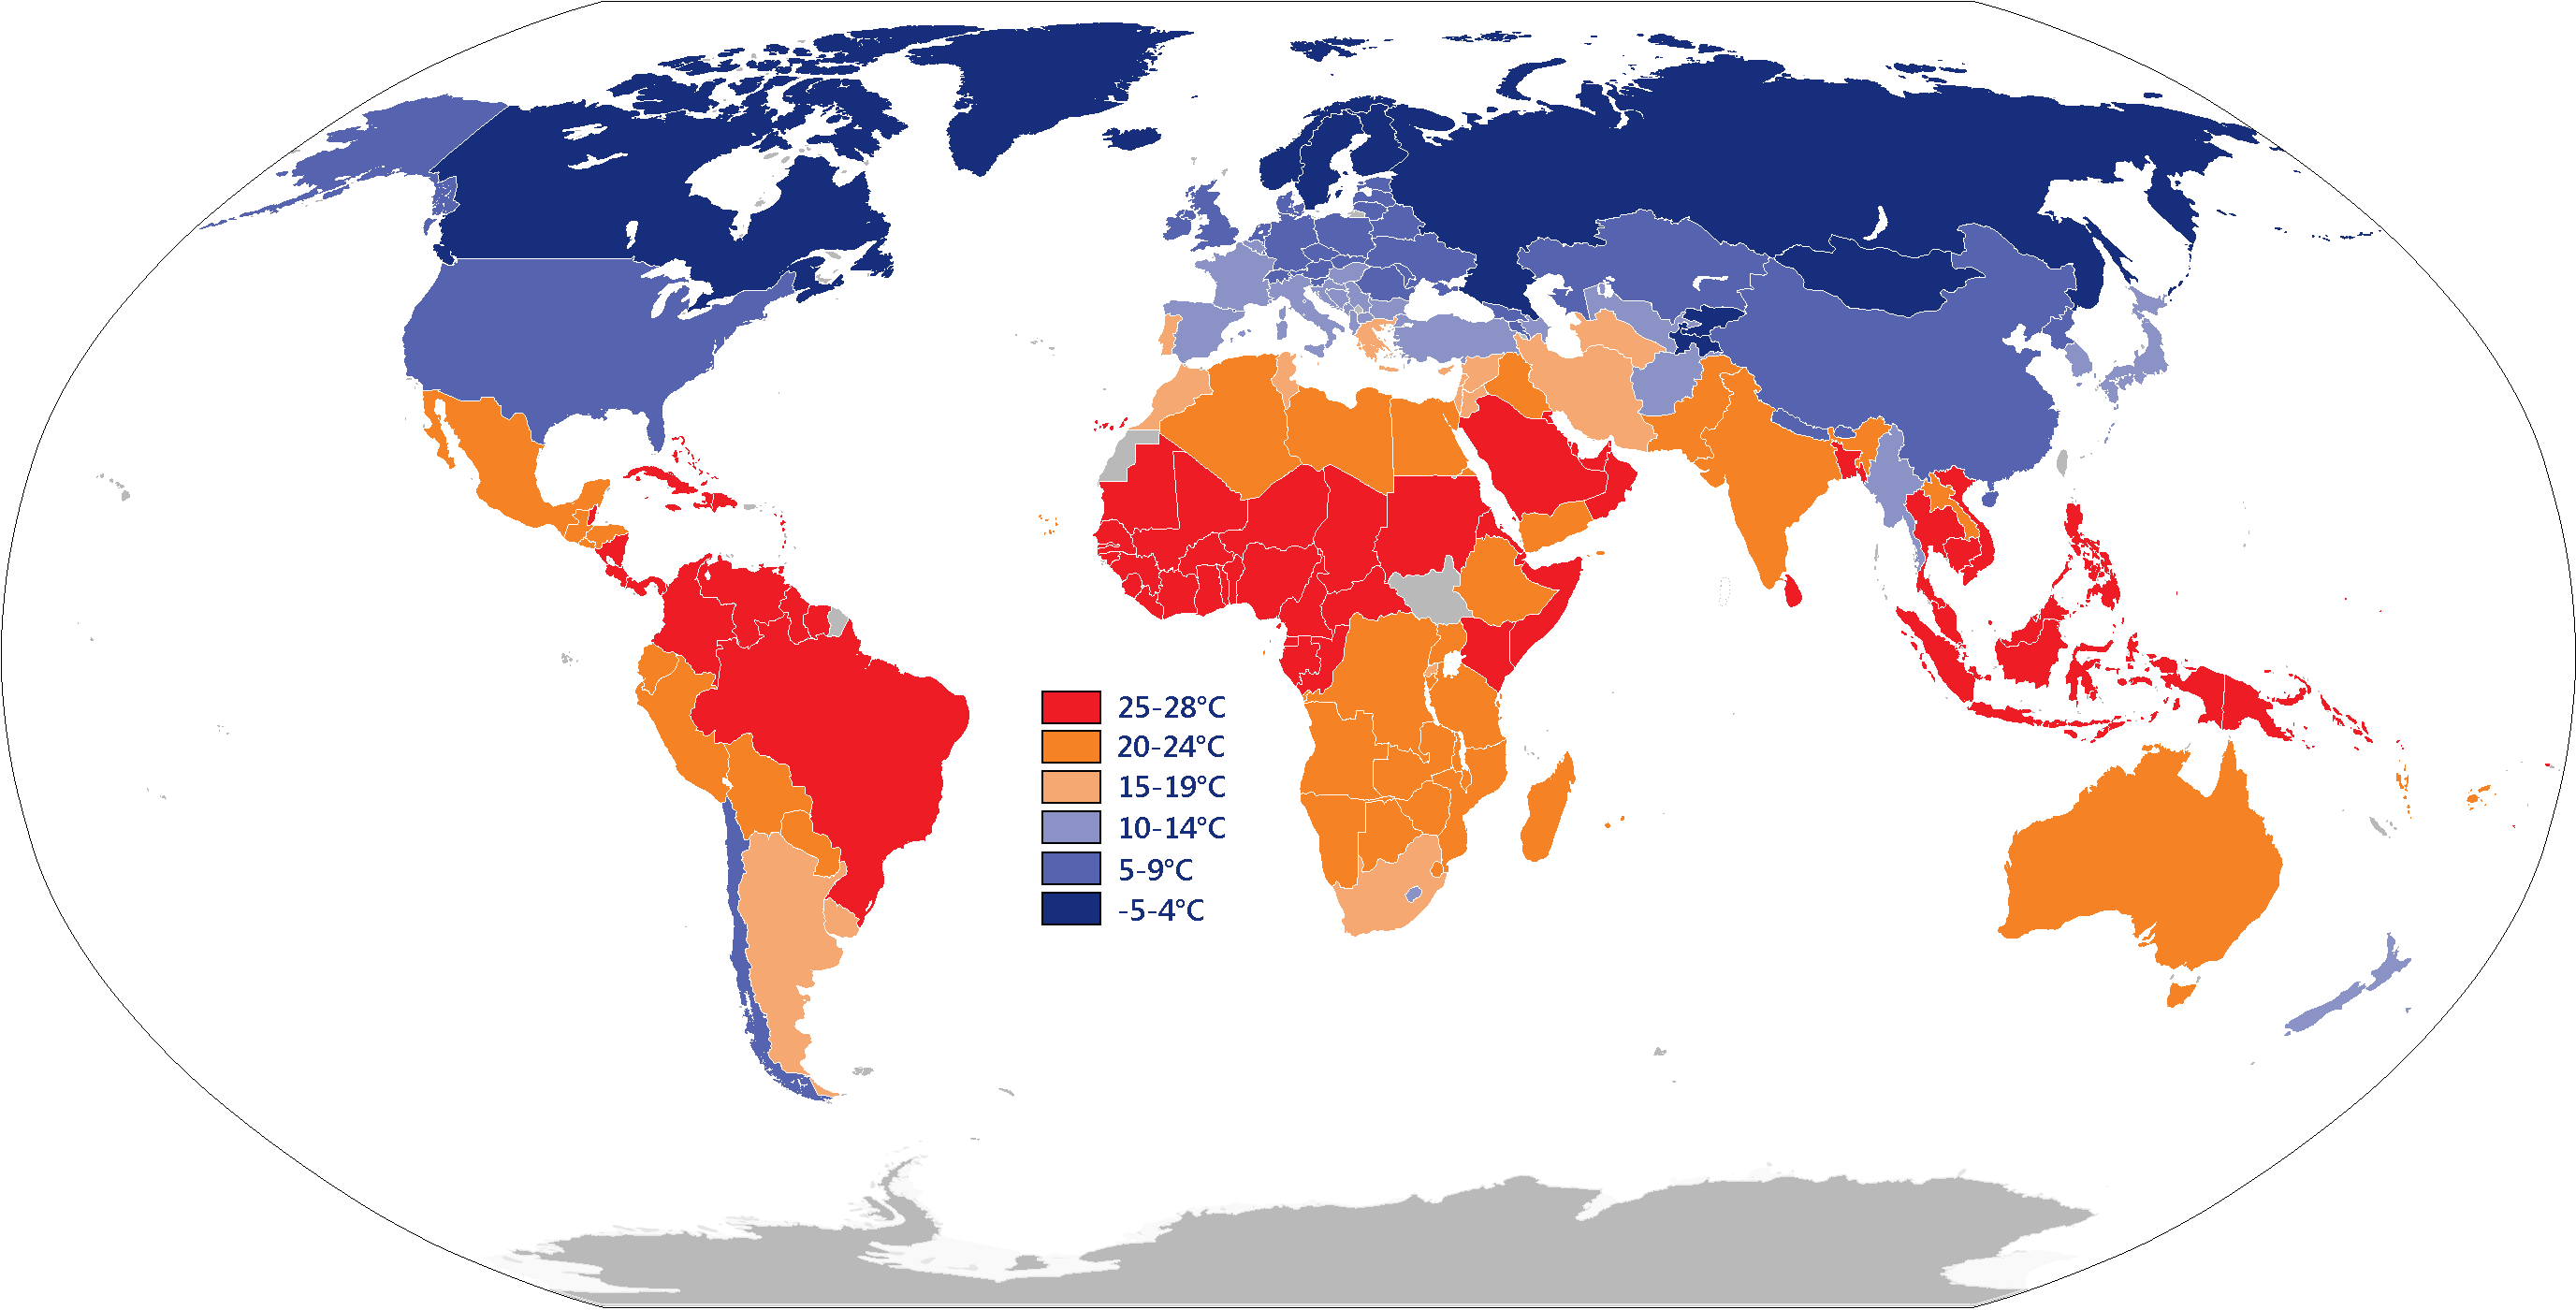
\includegraphics[width=0.9\linewidth]{images/Average_yearly_temperature_per_country.png}
	\caption{Average Temperatures for countries.}
	\label{fig:worldtemperature}
\end{figure}
The temperatures don't go higher than 30$\degree$C on Figure \ref{fig:worldtemperature}, but there may be local regions where the temperature is hotter than 30$\degree$C during certain periods of the year.
\\\\
Due to climate change, the low temperatures in many northern countries will rise in the following decades. This means that the component may be able to be deployed up north. 
\section{Conclusions}
To conclude, we will recommend different methods based off their run time and storage size.\\The fastest methods are the full storage, packed storage and the band storage which are all solved by Cholesky factorisation, then forward substitution, and backwards substitution. Band storage also requires the least amount of storage comparatively to the other storages that use direct methods. Therefore, as Band storage is the most efficient storage method as it is both one of the fastest of both the direct and iterative methods and requires the least amount of memory out of all the direct methods. It is recommended that for problems in the future of a similar nature, band storage and cholesky factorisation is recommended as providing the greatest efficiency.
\pagebreak
\section{Appendices}
\subsection*{Appendix A}
\begin{align*}
2\text{T}_0-\text{T}_1-\text{T}_6              & =0\\
3\text{T}_1-\text{T}_0-\text{T}_2-\text{T}_7          & =0\\
3\text{T}_2-\text{T}_1-\text{T}_3-\text{T}_8          & =0\\
3\text{T}_3-\text{T}_2-\text{T}_4-\text{T}_9          & =0\\
3\text{T}_4-\text{T}_3-\text{T}_5-\text{T}_{10}       & =0\\
3\text{T}_5-\text{T}_4-\text{T}_{11}           & =40\\
3\text{T}_6-\text{T}_0-\text{T}_7-\text{T}_{12}       & =0\\
4\text{T}_7-\text{T}_8-\text{T}_1-\text{T}_6-\text{T}_{13}   & =0\\
4\text{T}_8-\text{T}_7-\text{T}_2-\text{T}_9-\text{T}_{14}   & =0\\
4\text{T}_9-\text{T}_8-\text{T}_3-\text{T}_{10}-\text{T}_{15}& =0\\
4\text{T}_{10}-\text{T}_9-\text{T}_4-\text{T}_{11}-\text{T}_{16} & =0\\
4\text{T}_{11}-\text{T}_{10}-\text{T}_5-\text{T}_{17} & =40\\
3\text{T}_{12}-\text{T}_6-\text{T}_{16}-\text{T}_{13} & =0\\
4\text{T}_{13}-\text{T}_{12}-\text{T}_{14}-\text{T}_{7}-\text{T}_{19} & =0\\
4\text{T}_{14}-\text{T}_{13}-\text{T}_{15}-\text{T}_{8}-\text{T}_{20} & =0\\
4\text{T}_{15}-\text{T}_{14}-\text{T}_{16}-\text{T}_{9}-\text{T}_{21} & =0\\
4\text{T}_{16}-\text{T}_{15}-\text{T}_{17}-\text{T}_{10}-\text{T}_{22}& =0\\
4\text{T}_{17}-\text{T}_{16}-\text{T}_{11}-\text{T}_{23} & =40\\
3\text{T}_{18}-\text{T}_{12}-\text{T}_{24}-\text{T}_{19} & =0\\
4\text{T}_{19}-\text{T}_{18}-\text{T}_{20}-\text{T}_{13}-\text{T}_{25} & =0\\
4\text{T}_{20}-\text{T}_{19}-\text{T}_{21}-\text{T}_{14}-\text{T}_{26} & =0\\
4\text{T}_{21}-\text{T}_{20}-\text{T}_{22}-\text{T}_{15}-\text{T}_{27} & =0\\
4\text{T}_{22}-\text{T}_{21}-\text{T}_{23}-\text{T}_{16}-\text{T}_{28} & =0\\
\bigg(2+\frac{0.2\sqrt{2}}{3}\bigg)\text{T}_{23}-\text{T}_{22}-\text{T}_{17} & =\frac{4\sqrt{2}}{3}\\
3\text{T}_{24}-\text{T}_{18}-\text{T}{30}-\text{T}_{25} &=0\\
4\text{T}_{25}-\text{T}_{24}-\text{T}_{26}-\text{T}_{19}-\text{T}_{31} & =0\\
4\text{T}_{26}-\text{T}_{25}-\text{T}_{27}-\text{T}_{20}-\text{T}_{32} & =0\\
4\text{T}_{27}-\text{T}_{26}-\text{T}_{28}-\text{T}_{21}-\text{T}_{33} & =0\\
\bigg(2+\frac{0.2\sqrt{2}}{3}\bigg)\text{T}_{28}-\text{T}_{27}-\text{T}_{22} & =\frac{4\sqrt{2}}{3}\\
\text{T}_{29} \text{ is null}\\
3\text{T}_{30}-\text{T}_{24}-\text{T}_{31} &=70\\
4\text{T}_{31}-\text{T}_{30}-\text{T}_{32}-\text{T}_{25} &=70\\
4\text{T}_{32}-\text{T}_{31}-\text{T}_{33}-\text{T}_{26} &=70\\
\bigg(2+\frac{0.2\sqrt{2}}{3}\bigg)\text{T}_{33}-\text{T}_{32}-\text{T}_{27} & =\frac{4\sqrt{2}}{3}\\
\text{T}_{34} \text{ is null}\\
\text{T}_{35} \text{ is null}
\end{align*}
\subsection*{Appendix B}
\begin{figure}[H]
	\centering
	\begin{subfigure}[b]{0.48\textwidth}
		\centering
		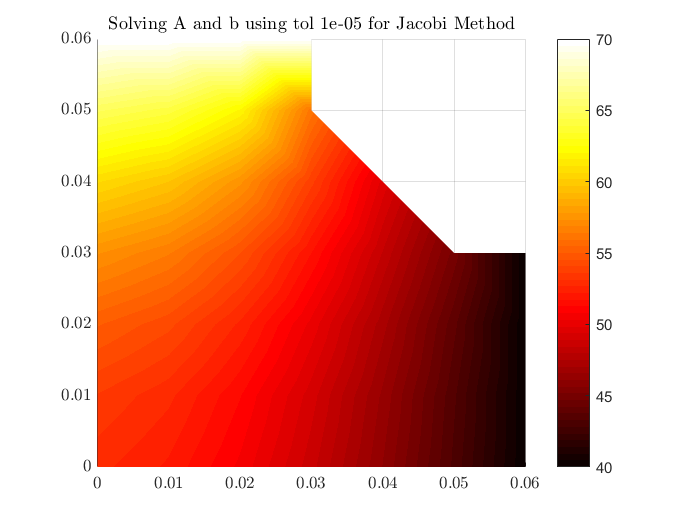
\includegraphics[width=\linewidth]{images/JacobiComparisontole-05.png}
		\caption{Tolerance of $10^{-5}$.}
		\label{fig:Jacobitole-05}
	\end{subfigure}
	\hfill
	\begin{subfigure}[b]{0.48\textwidth}
		\centering
		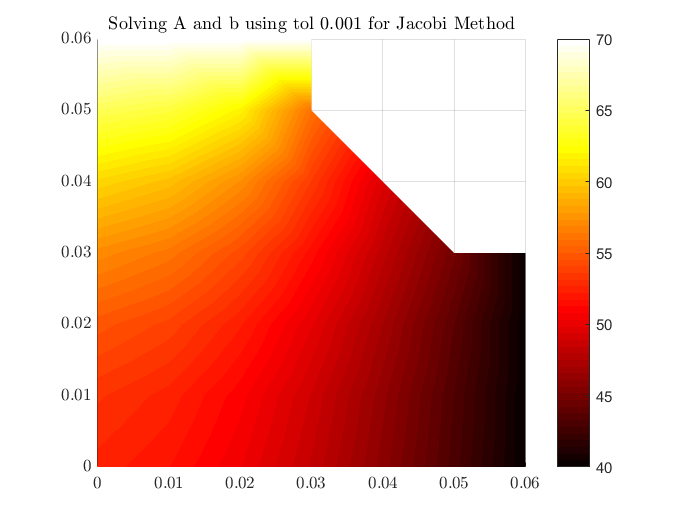
\includegraphics[width=\linewidth]{images/JacobiComparisontol0-001.png}
		\caption{Tolerance of $10^{-3}$.}
		\label{fig:Jacobitol0.001}
	\end{subfigure}
	\hfill
	\begin{subfigure}[b]{0.48\textwidth}
		\centering
		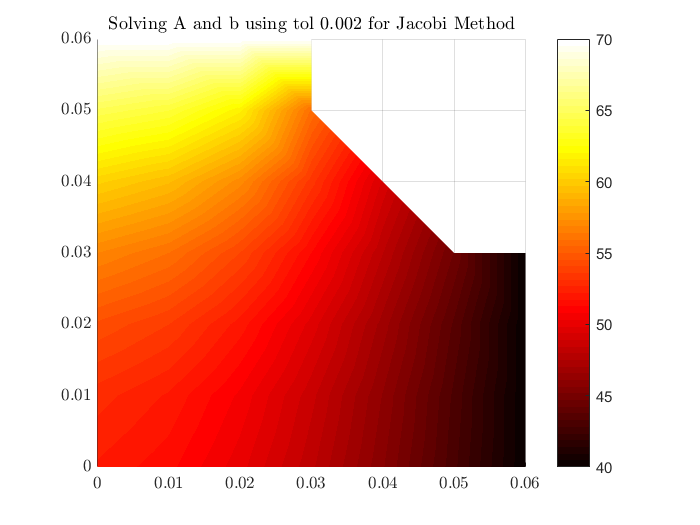
\includegraphics[width=\linewidth]{images/JacobiComparisontol0-002.png}
		\caption{Tolerance of $2 \times 10^{-3}$.}
		\label{fig:Jacobitol0.002}
	\end{subfigure}
	\hfill
	\begin{subfigure}[b]{0.48\textwidth}
		\centering
		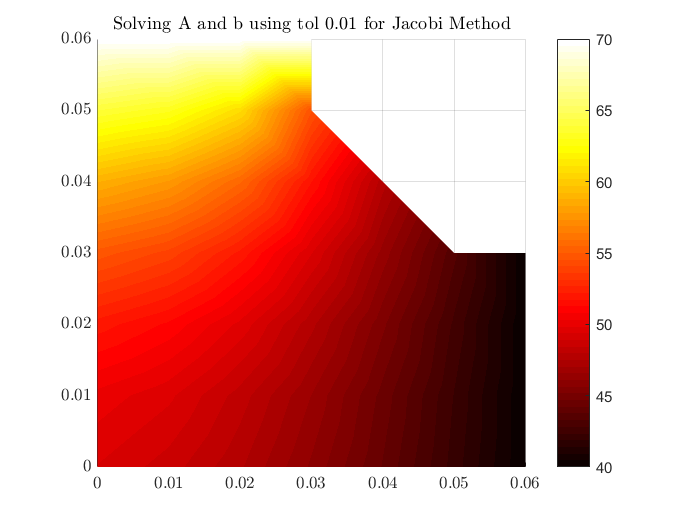
\includegraphics[width=\linewidth]{images/JacobiComparisontol0-01.png}
		\caption{Tolerance of $10^{-2}$.}
		\label{fig:Jacobitol0.01}
	\end{subfigure}
	\hfill
	\begin{subfigure}[b]{0.48\textwidth}
		\centering
		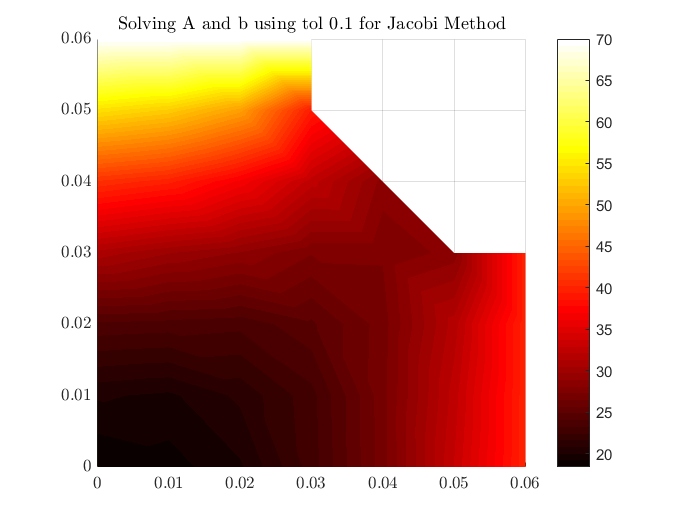
\includegraphics[width=\linewidth]{images/JacobiComparisontol0-1.png}
		\caption{Tolerance of $10^{-1}$.}
		\label{fig:Jacobitol0.1}
	\end{subfigure}
	\hfill
	\begin{subfigure}[b]{0.48\textwidth}
		\centering
		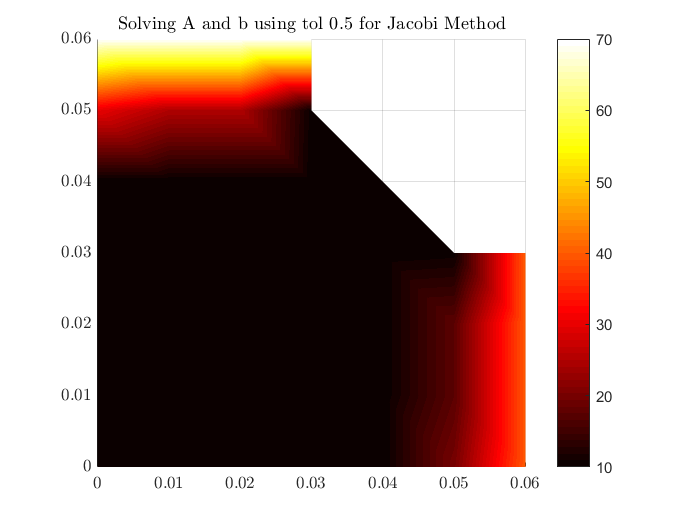
\includegraphics[width=\linewidth]{images/JacobiComparisontol0-5.png}
		\caption{Tolerance of $0.5$.}
		\label{fig:Jacobitol0.5}
	\end{subfigure}
	\caption{Varying tolerances for solving $x$ using the Jacobi Method.}
    \label{fig:Jacobitolerance}
\end{figure}

\begin{figure}[H]
	\centering
	\begin{subfigure}[b]{0.48\textwidth}
		\centering
		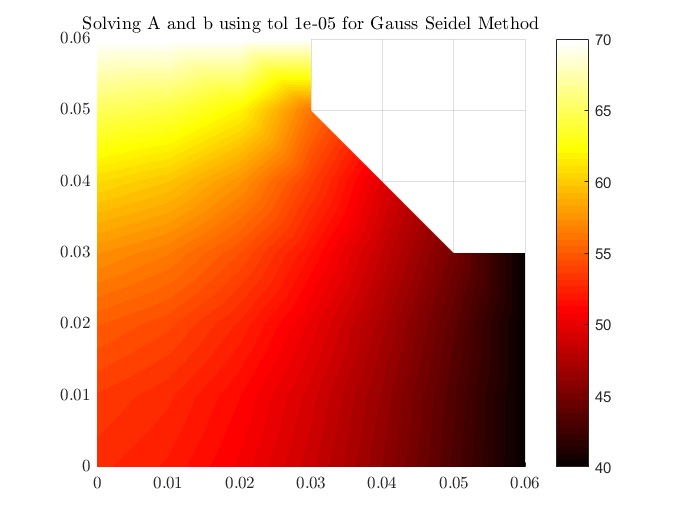
\includegraphics[width=\linewidth]{images/GaussComparisontole-05.png}
		\caption{Tolerance of $10^{-5}$.}
		\label{fig:Gausstole-05}
	\end{subfigure}
	\hfill
	\begin{subfigure}[b]{0.48\textwidth}
		\centering
		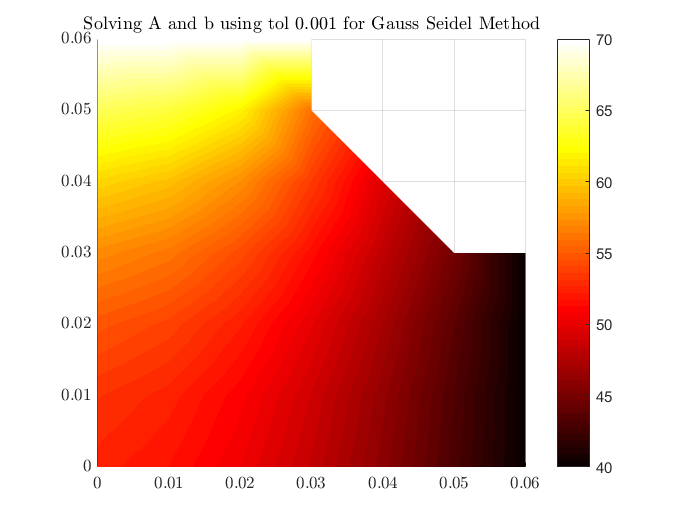
\includegraphics[width=\linewidth]{images/GaussComparisontol0-001.png}
		\caption{Tolerance of $10^{-3}$.}
		\label{fig:Gausstol0.001}
	\end{subfigure}
	\hfill
	\begin{subfigure}[b]{0.48\textwidth}
		\centering
		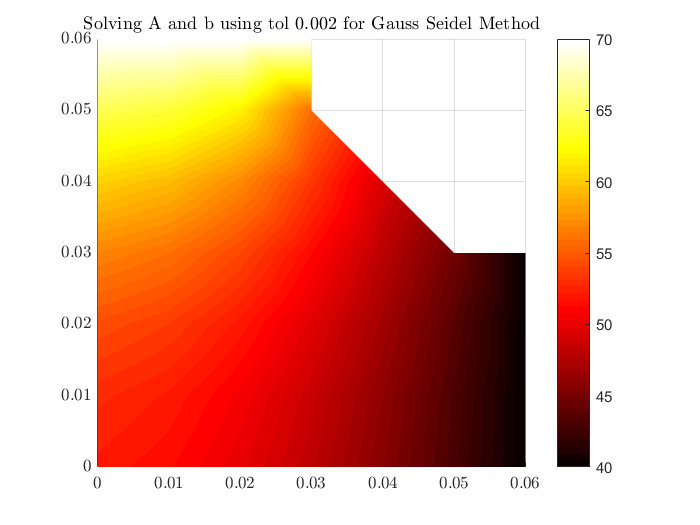
\includegraphics[width=\linewidth]{images/GaussComparisontol0-002.png}
		\caption{Tolerance of $2 \times 10^{-3}$.}
		\label{fig:Gausstol0.002}
	\end{subfigure}
	\hfill
	\begin{subfigure}[b]{0.48\textwidth}
		\centering
		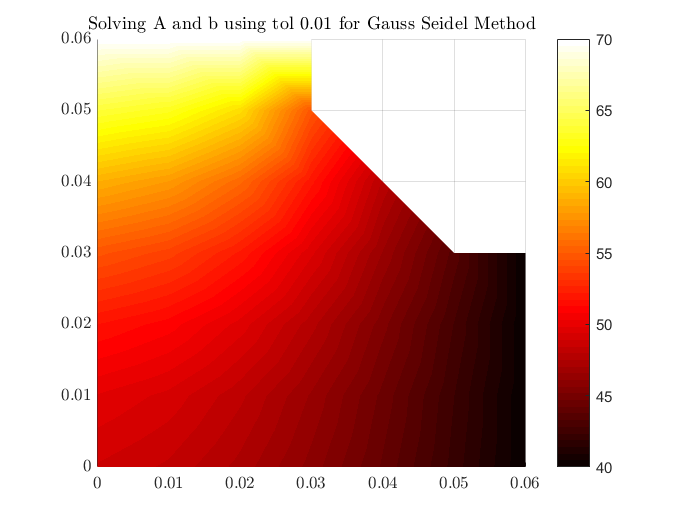
\includegraphics[width=\linewidth]{images/GaussComparisontol0-01.png}
		\caption{Tolerance of $10^{-2}$.}
		\label{fig:Gausstol0.01}
	\end{subfigure}
	\hfill
	\begin{subfigure}[b]{0.48\textwidth}
		\centering
		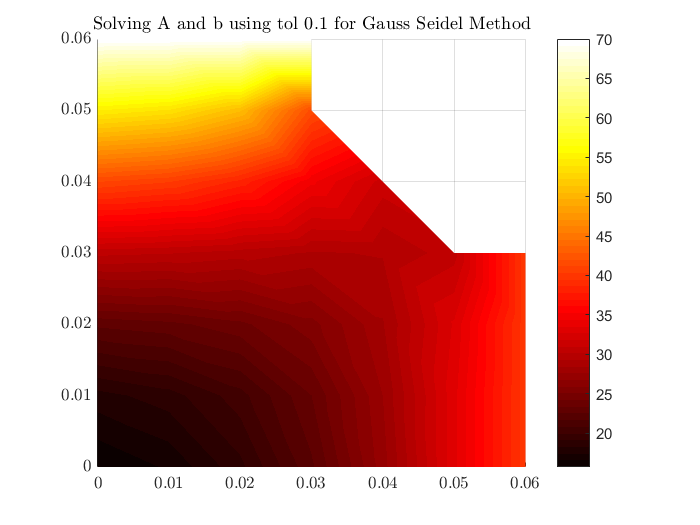
\includegraphics[width=\linewidth]{images/GaussComparisontol0-1.png}
		\caption{Tolerance of $10^{-1}$.}
		\label{fig:tol0.1}
	\end{subfigure}
	\hfill
	\begin{subfigure}[b]{0.48\textwidth}
		\centering
		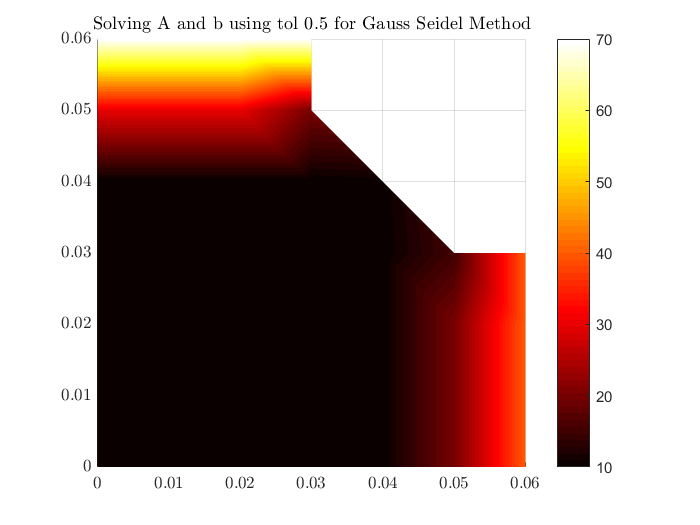
\includegraphics[width=\linewidth]{images/GaussComparisontol0-5.png}
		\caption{Tolerance of $0.5$.}
		\label{fig:Gausstol0.5}
	\end{subfigure}
	\caption{Varying tolerances for solving $x$ using the Gauss-Seidel Method.}
    \label{fig:Gausstolerance}
\end{figure}

\begin{figure}[H]
	\centering
	\begin{subfigure}[b]{0.48\textwidth}
		\centering
		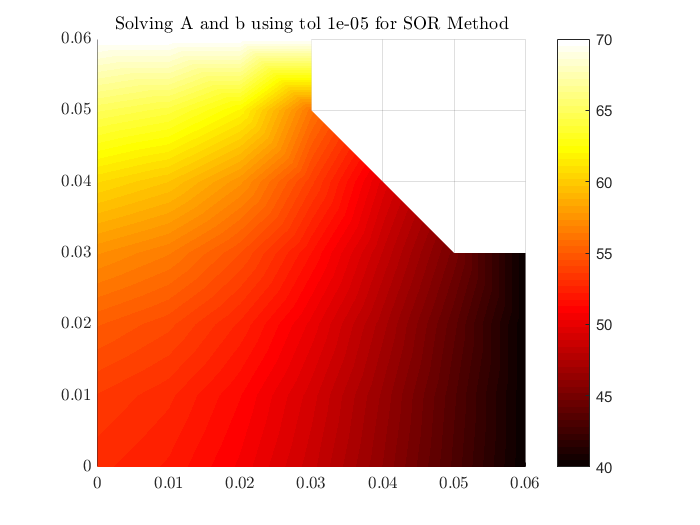
\includegraphics[width=\linewidth]{images/SORComparisontole-05.png}
		\caption{Tolerance of $10^{-5}$.}
		\label{fig:SORtole-05}
	\end{subfigure}
	\hfill
	\begin{subfigure}[b]{0.48\textwidth}
		\centering
		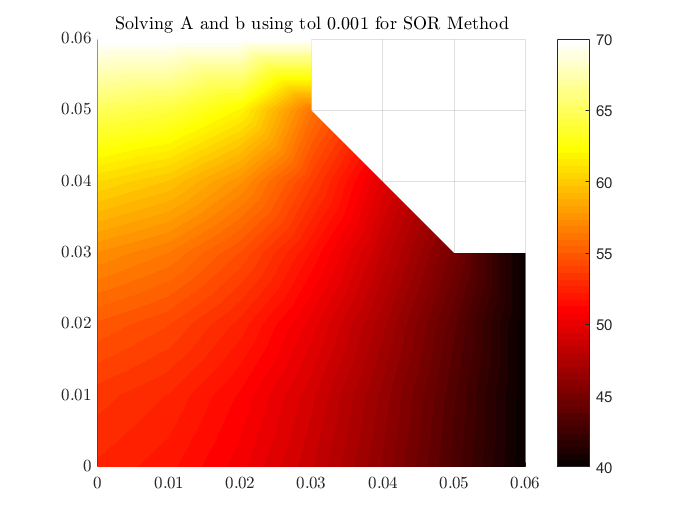
\includegraphics[width=\linewidth]{images/SORComparisontol0-001.png}
		\caption{Tolerance of $10^{-3}$.}
		\label{fig:SORtol0.001}
	\end{subfigure}
	\hfill
	\begin{subfigure}[b]{0.48\textwidth}
		\centering
		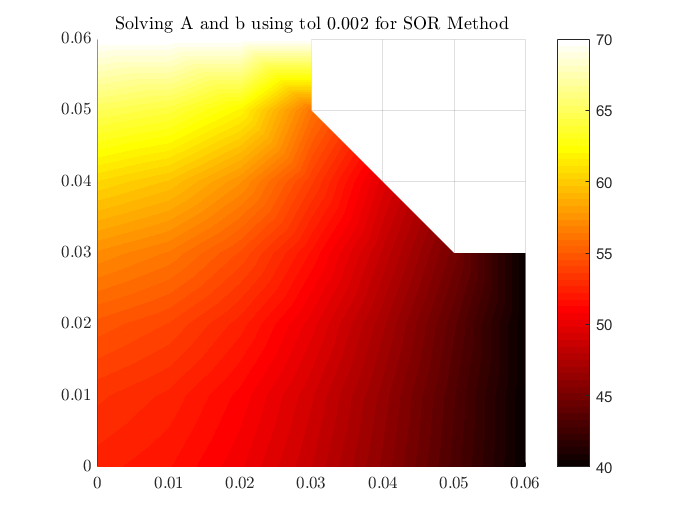
\includegraphics[width=\linewidth]{images/SORComparisontol0-002.png}
		\caption{Tolerance of $2 \times 10^{-3}$.}
		\label{fig:SORtol0.002}
	\end{subfigure}
	\hfill
	\begin{subfigure}[b]{0.48\textwidth}
		\centering
		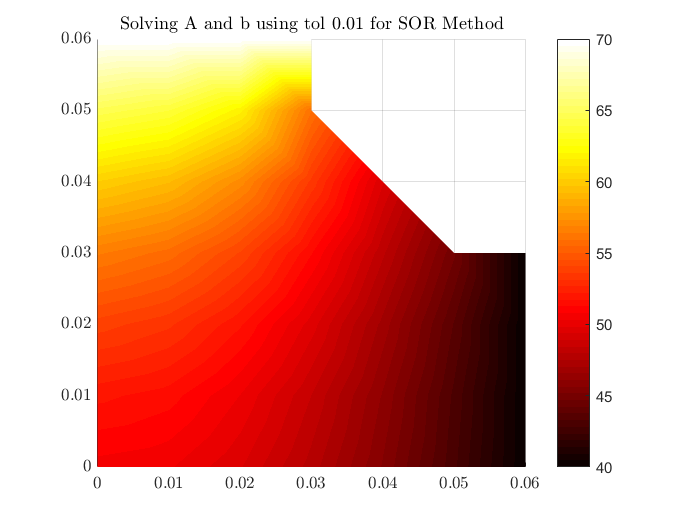
\includegraphics[width=\linewidth]{images/SORComparisontol0-01.png}
		\caption{Tolerance of $10^{-2}$.}
		\label{fig:SORtol0.01}
	\end{subfigure}
	\hfill
	\begin{subfigure}[b]{0.48\textwidth}
		\centering
		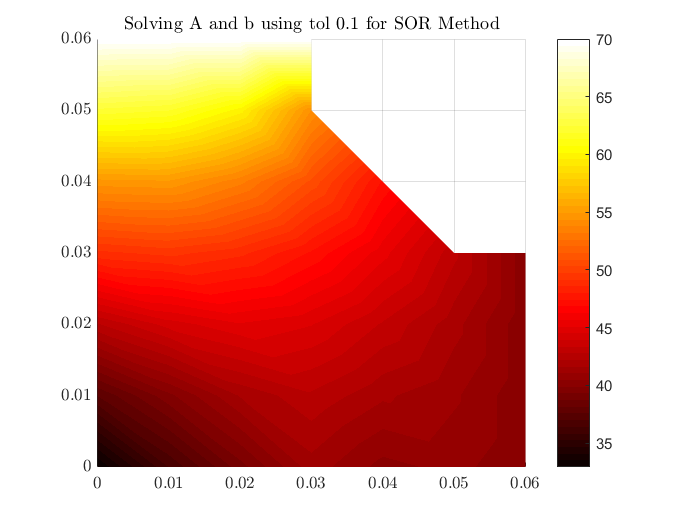
\includegraphics[width=\linewidth]{images/SORComparisontol0-1.png}
		\caption{Tolerance of $10^{-1}$.}
		\label{fig:SORtol0.1}
	\end{subfigure}
	\hfill
	\begin{subfigure}[b]{0.48\textwidth}
		\centering
		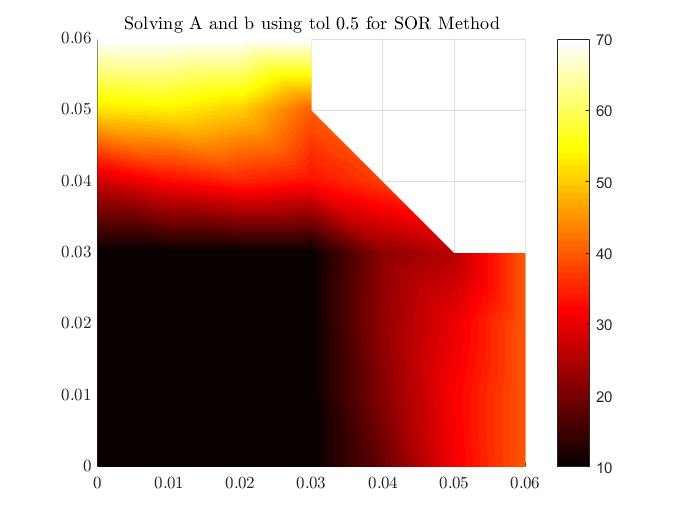
\includegraphics[width=\linewidth]{images/SORComparisontol0-5.png}
		\caption{Tolerance of $0.5$.}
		\label{fig:SORtol0.5}
	\end{subfigure}
	\caption{Varying tolerances for solving $x$ using the SOR Method.}
    \label{fig:SORtolerance}
\end{figure}

\begin{figure}[H]
	\centering
	\begin{subfigure}[b]{0.48\textwidth}
		\centering
		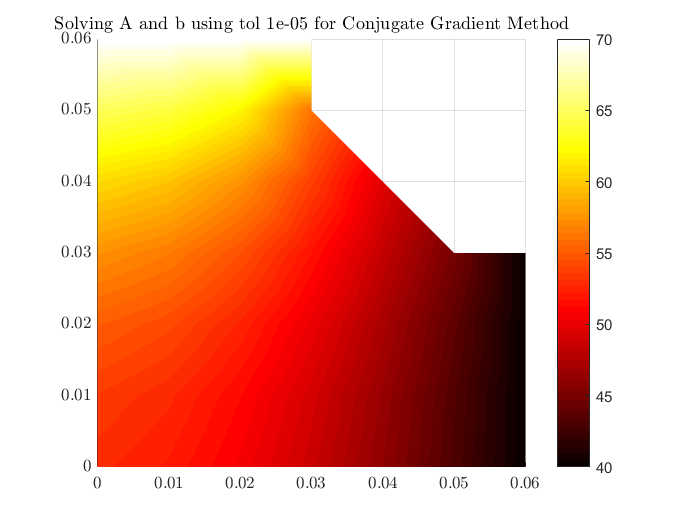
\includegraphics[width=\linewidth]{images/ConjugateComparisontole-05.png}
		\caption{Tolerance of $10^{-5}$.}
		\label{fig:Conjugatetole-05}
	\end{subfigure}
	\hfill
	\begin{subfigure}[b]{0.48\textwidth}
		\centering
		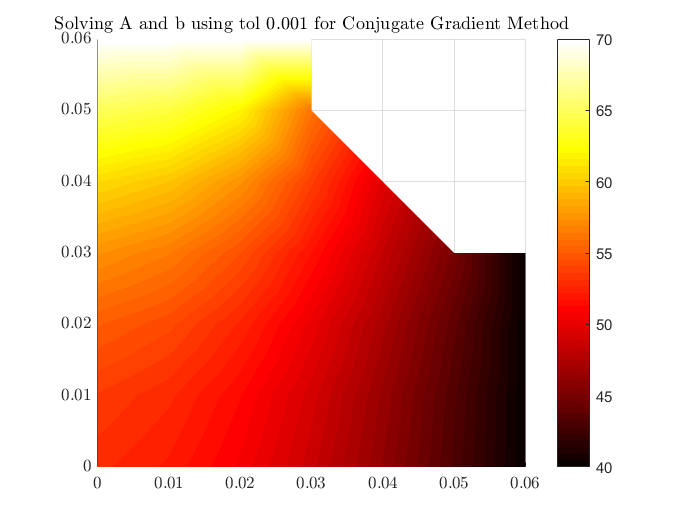
\includegraphics[width=\linewidth]{images/ConjugateComparisontol0-001.png}
		\caption{Tolerance of $10^{-3}$.}
		\label{fig:Conjugatetol0.001}
	\end{subfigure}
	\hfill
	\begin{subfigure}[b]{0.48\textwidth}
		\centering
		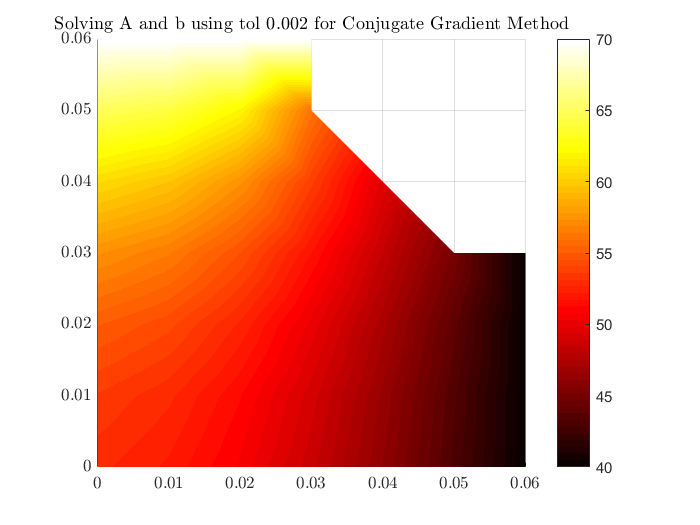
\includegraphics[width=\linewidth]{images/ConjugateComparisontol0-002.png}
		\caption{Tolerance of $2 \times 10^{-3}$.}
		\label{fig:Conjugatetol0.002}
	\end{subfigure}
	\hfill
	\begin{subfigure}[b]{0.48\textwidth}
		\centering
		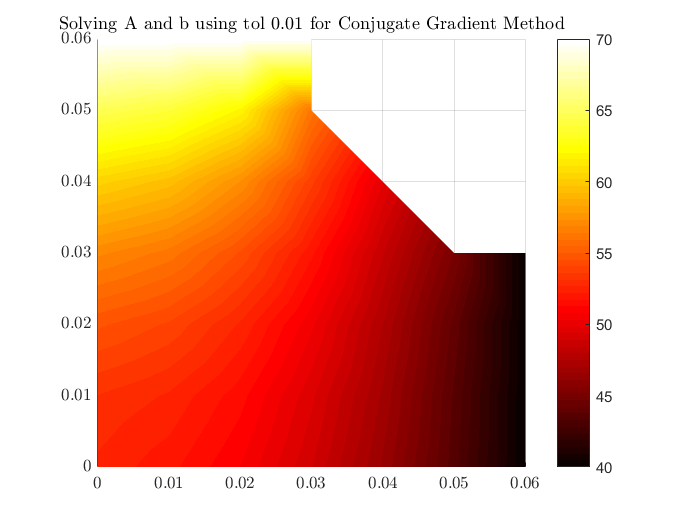
\includegraphics[width=\linewidth]{images/ConjugateComparisontol0-01.png}
		\caption{Tolerance of $10^{-2}$.}
		\label{fig:Conjugatetol0.01}
	\end{subfigure}
	\hfill
	\begin{subfigure}[b]{0.48\textwidth}
		\centering
		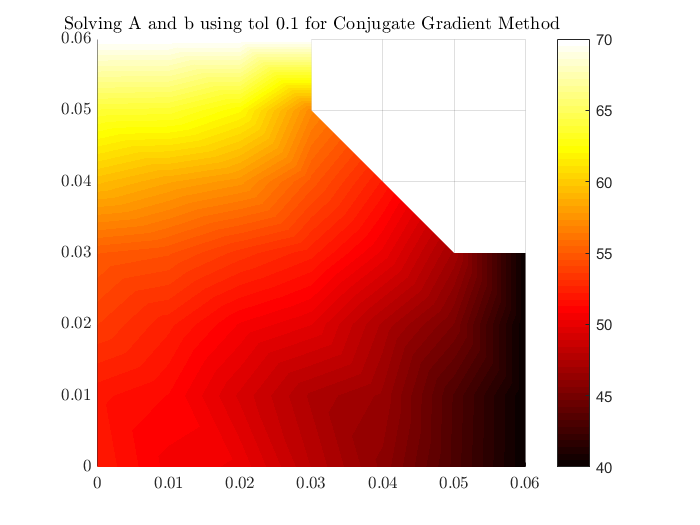
\includegraphics[width=\linewidth]{images/ConjugateComparisontol0-1.png}
		\caption{Tolerance of $10^{-1}$.}
		\label{fig:Conjugatetol0.1}
	\end{subfigure}
	\hfill
	\begin{subfigure}[b]{0.48\textwidth}
		\centering
		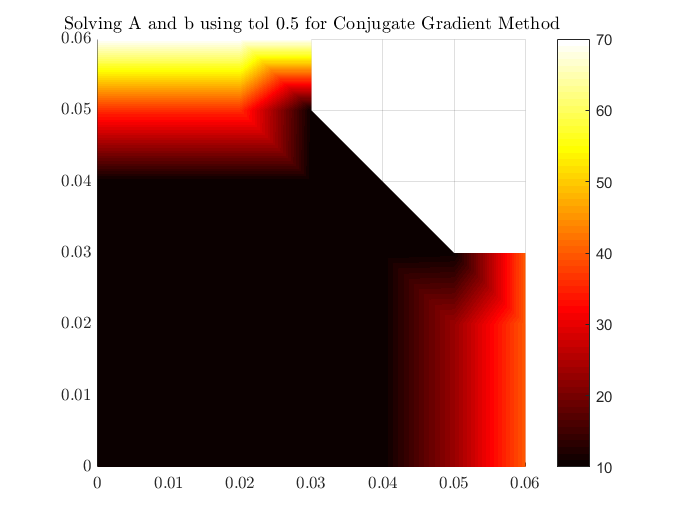
\includegraphics[width=\linewidth]{images/ConjugateComparisontol0-5.png}
		\caption{Tolerance of $0.5$.}
		\label{fig:Conjugatetol0.5}
	\end{subfigure}
	\caption{Varying tolerances for solving $x$ using the Conjugate Gradient Method.}
    \label{fig:tolerance}
\end{figure}

\end{document}